\documentclass[paper=a4,fontsize=12pt,ngerman]{scrartcl}

\usepackage[utf8]{inputenc}				
\usepackage[T1]{fontenc}
\usepackage{float}
\usepackage{graphicx}
\usepackage{tabularx}
\usepackage{subcaption}
\usepackage[english]{babel}
\usepackage{amsmath}
\usepackage[a4paper,left=25mm,right=35mm,top=25mm,bottom=30mm]{geometry}
\usepackage{listings}
\usepackage{xcolor}
\usepackage{url}
\usepackage{hyperref}
\usepackage[expansion=false]{microtype}
\usepackage{pdfpages}
\usepackage{caption}

\geometry{a4paper, margin=1in}

\lstset{ basicstyle=\ttfamily\footnotesize,
keywordstyle=\color{blue},  commentstyle=\color{green!50!black},
  stringstyle=\color{red},
  frame=single, 
  breaklines=true,
  showstringspaces=false
}

\graphicspath{{graphics/}}

\begin{document}

\pagenumbering{roman}
\pagestyle{plain}

% Einbinden der Titelseite
\begin{titlepage}

\linespread{1.5}


\includegraphics[width=\linewidth]{graphics/htw_logo}

\begin{center}
    \large  
    \hfill
    \vfill
    \Large{\bfseries{OASIS: Optimized Aqua Soil Irrigation System}}
    
    By \\
    Micha{\l} Roziel, 5012845\\
    Hanan Ahmed Ashir, 5012967 \\
    Laith Arafeh, 5024761\\
    Omar Qoul, 5024765

    \vfill
	%A low-cost IoT solution that automates plant watering by measuring soil moisture and water tank levels and visualizing the data in real time. 
	
    \vfill	
    \vfill
	
    Saarbrücken, 04.02.2026
\end{center}
    
\end{titlepage}


% Hier ist der Abstract

% Das Inhaltsverzeichnis
\clearpage
\tableofcontents 

\clearpage
\pagenumbering{arabic}

\section{Introduction}

\subsection{Motivation}
Manual plant irrigation is often inefficient and inconsistent in practice. Irregular watering intervals or incorrectly estimated water quantities can lead to either resource wastage or an undersupply of water to the plants. 

Furthermore, rainwater frequently remains unutilized, as manual extraction and distribution from water containers is a labor-intensive work. From a computer science perspective, this problem presents an ideal application for an IoT control system designed to eliminate these inefficiencies through automation and data-driven decision-making.

\subsection{Project Description and Goals}
The project \emph{OASIS} consists of an ESP32-based sensor and a Raspberry-Pi acting as a central control unit. The primary objective of this project is to implement and test a cost-effective automation system. The focus lies on maximizing the utilization of rainwater.

The system is designed to ensure the following functionalities:

\begin{itemize}
    \item \textbf{Sensor Technology:} Deployment of two sensors to capture the system state. This includes measuring soil moisture as well as monitoring water levels.

    \item \textbf{Weather API:} Utilization of an open-source web API to verify recent rain levels. This ensures that watering is disabled if rainfall has occured within the past few hours, thereby preventing over-watering.
    
    \item \textbf{Automated Control:} The system autonomously regulates plant irrigation based on sensor data.

    \item \textbf{Overflow Management:} The system monitors the water level in the collection tank to detect and regulate potential overflows.
\end{itemize}
The data collected by the sensors and the ESP32 is stored locally on an InfluxDB, which can then be connected to a Grafana Dashboard, that visualizes the data.

\subsection{Scope}
The current scope of this project is limited to demonstrating the complete system logic using a miniaturized model. This model serves as a proof of concept, intended to validate the fundamental control logic and the technical architecture. The successful operation of this model forms the basis for scaling the system to a real-world garden.

\section{System Architecture and Technical Description}
To describe the structure of the OASIS System, a module based system architecture is used. This approach focuses on concrete hardware and software components and the communication between them. As a result, the actual system behavior and data flow are easier to understand and directly reflect the implemented solution. 


\begin{figure}[H]
    \centering
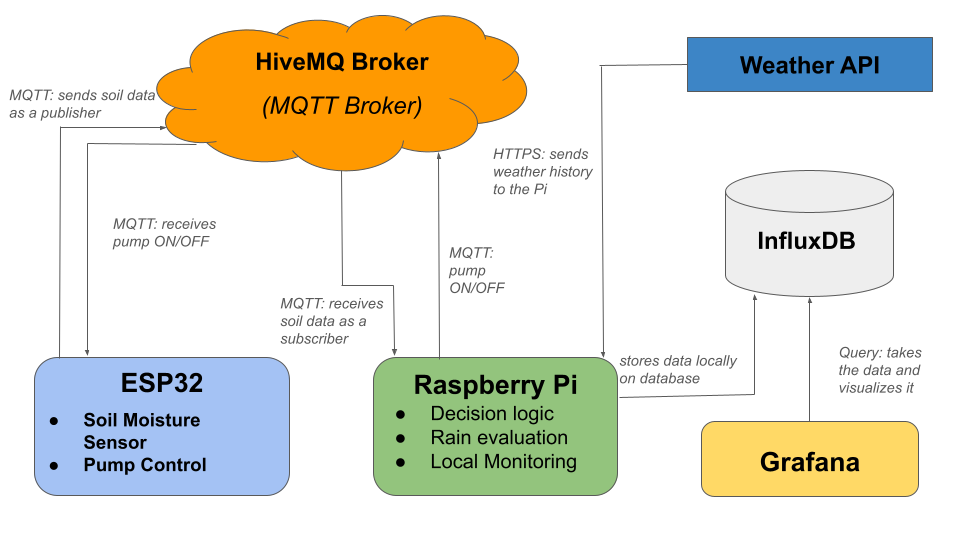
\includegraphics[width=0.75\linewidth]{graphics/Architecture_updated.png}
    \caption{Architecture of OASIS}
    \label{fig:placeholder}
\end{figure}

\subsection{Hardware Setup}
The hardware setup of the OASIS system consists of an ESP32 and a Raspberry Pi acting as the central control unit. The ESP32 is connected to a soil moisture sensor, which continuously measures the moisture level of the soil. The raw sensor values are processed locally on the ESP32 and converted into percentage based moisture readings.

In addition to sensing, the ESP32 controls a water pressure sensor and a water pump. Since the water pump operates at 12V and the water pressure sensor at 24V,  a relay and a amperage to voltage converter is used to isolate the microcontroller from the high voltage circuit and to safely switch the pump, since the ESP32 can only handle voltages up to 5V. This allows the system to physically execute irrigation actions based on received control commands. For monitoring and debugging purposes, the ESP32 outputs sensor readings to the serial monitor in real time.

\begin{figure}[H]
    \centering
    \begin{subfigure}[b]{0.49\textwidth}
        \centering
        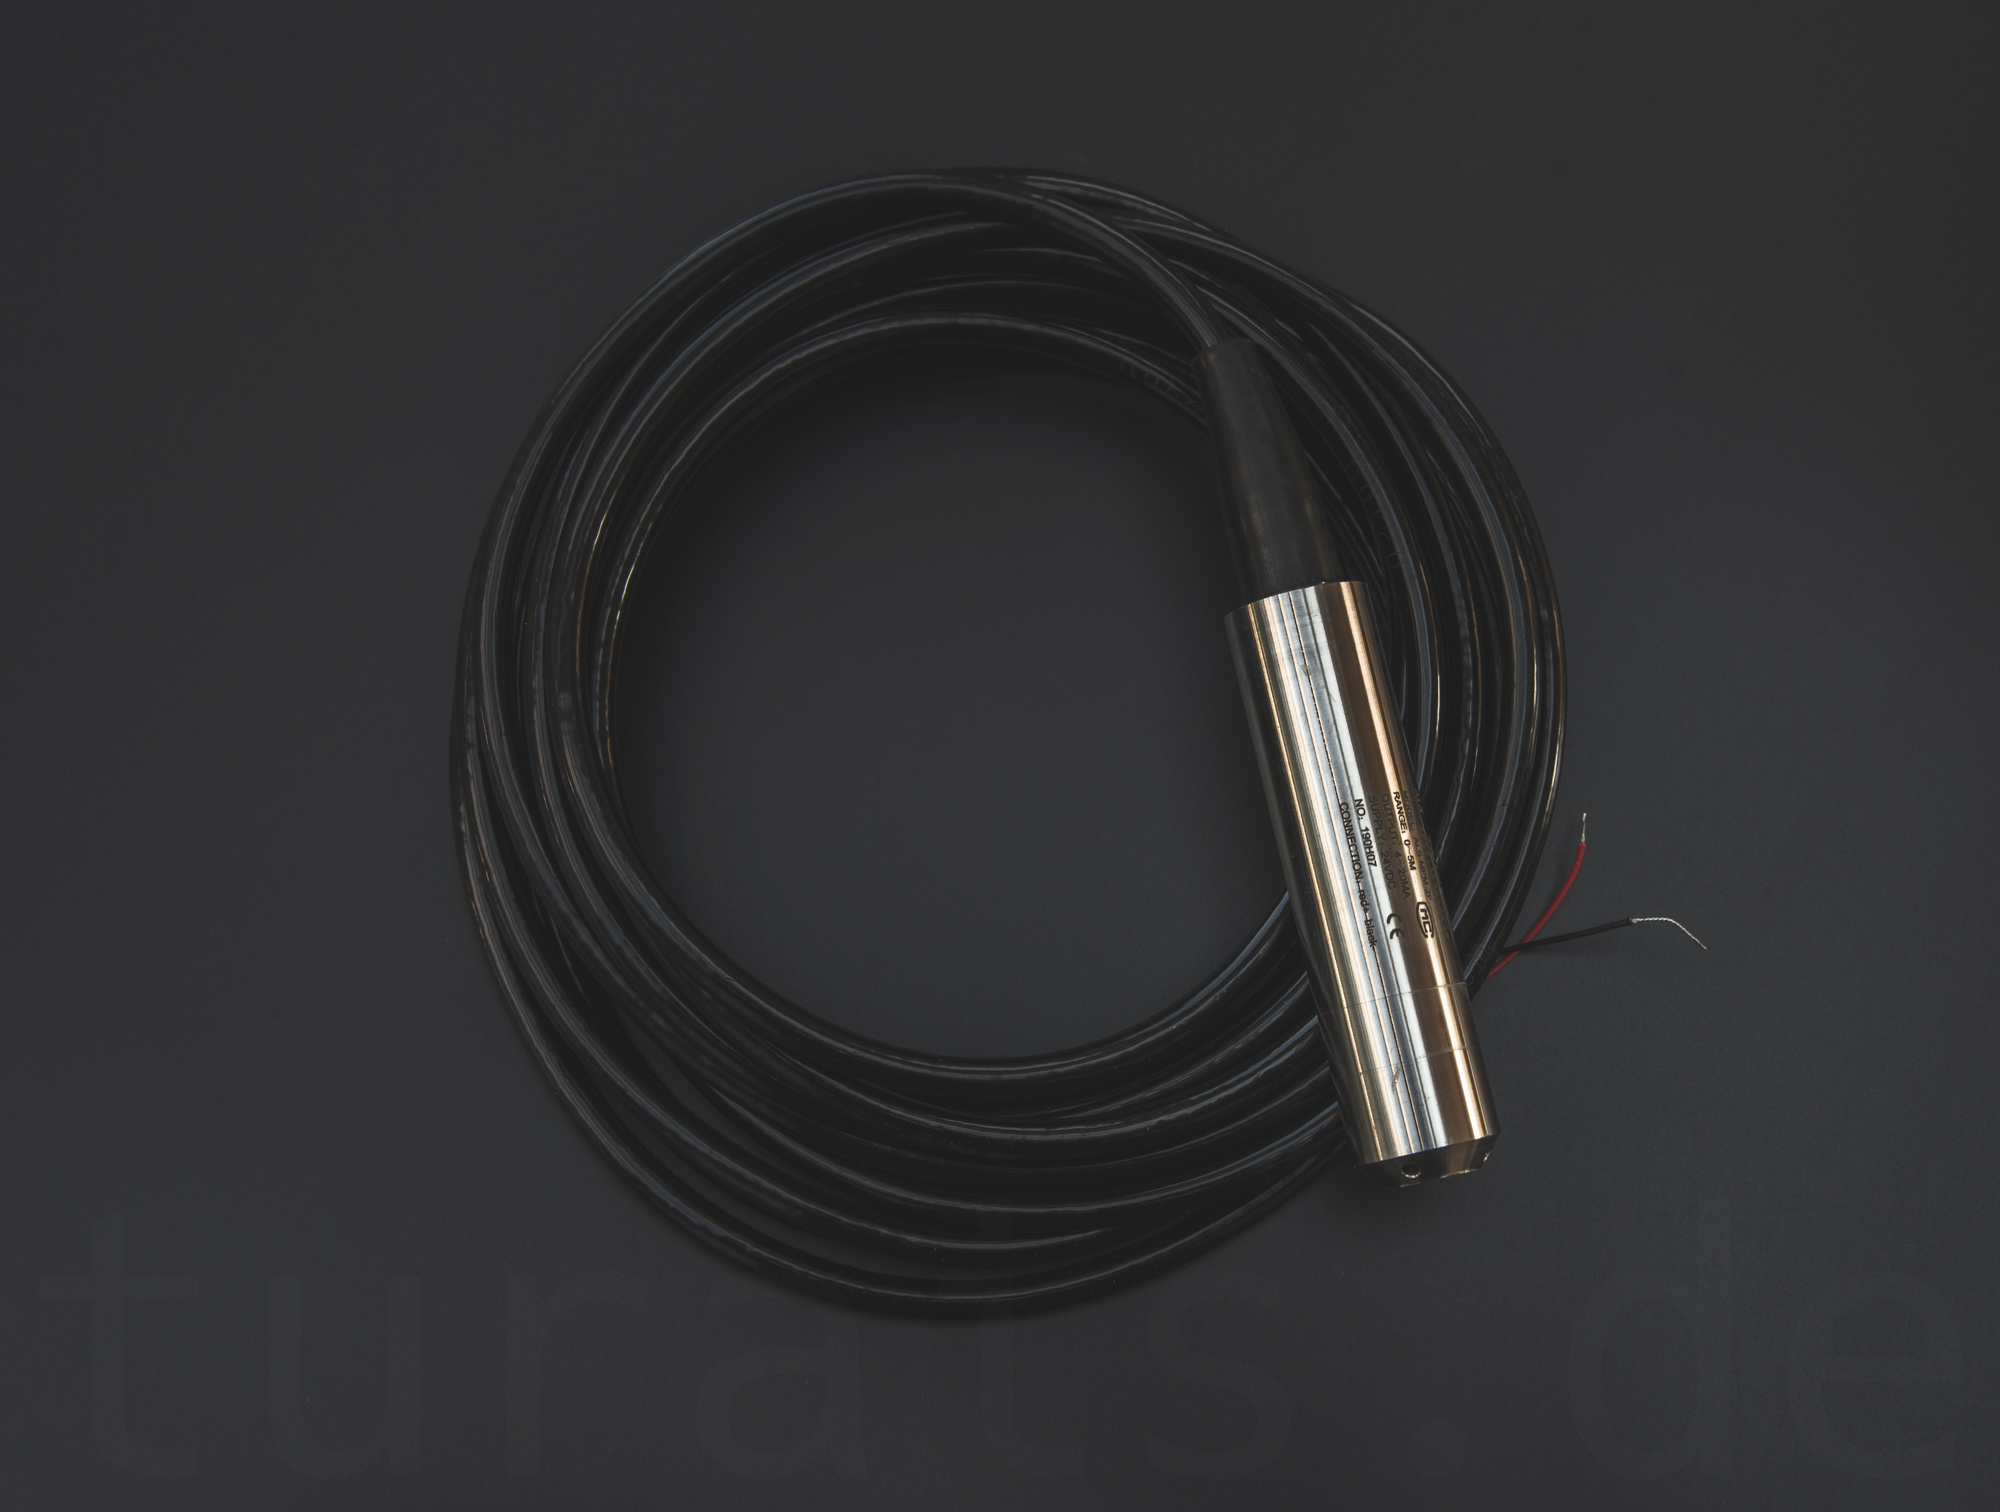
\includegraphics[width=\linewidth]{graphics/water_level_sensor.jpg}
        \caption{Water level Sensor}
    \end{subfigure}
    \hfill
    \begin{subfigure}[b]{0.49\textwidth}
        \centering
        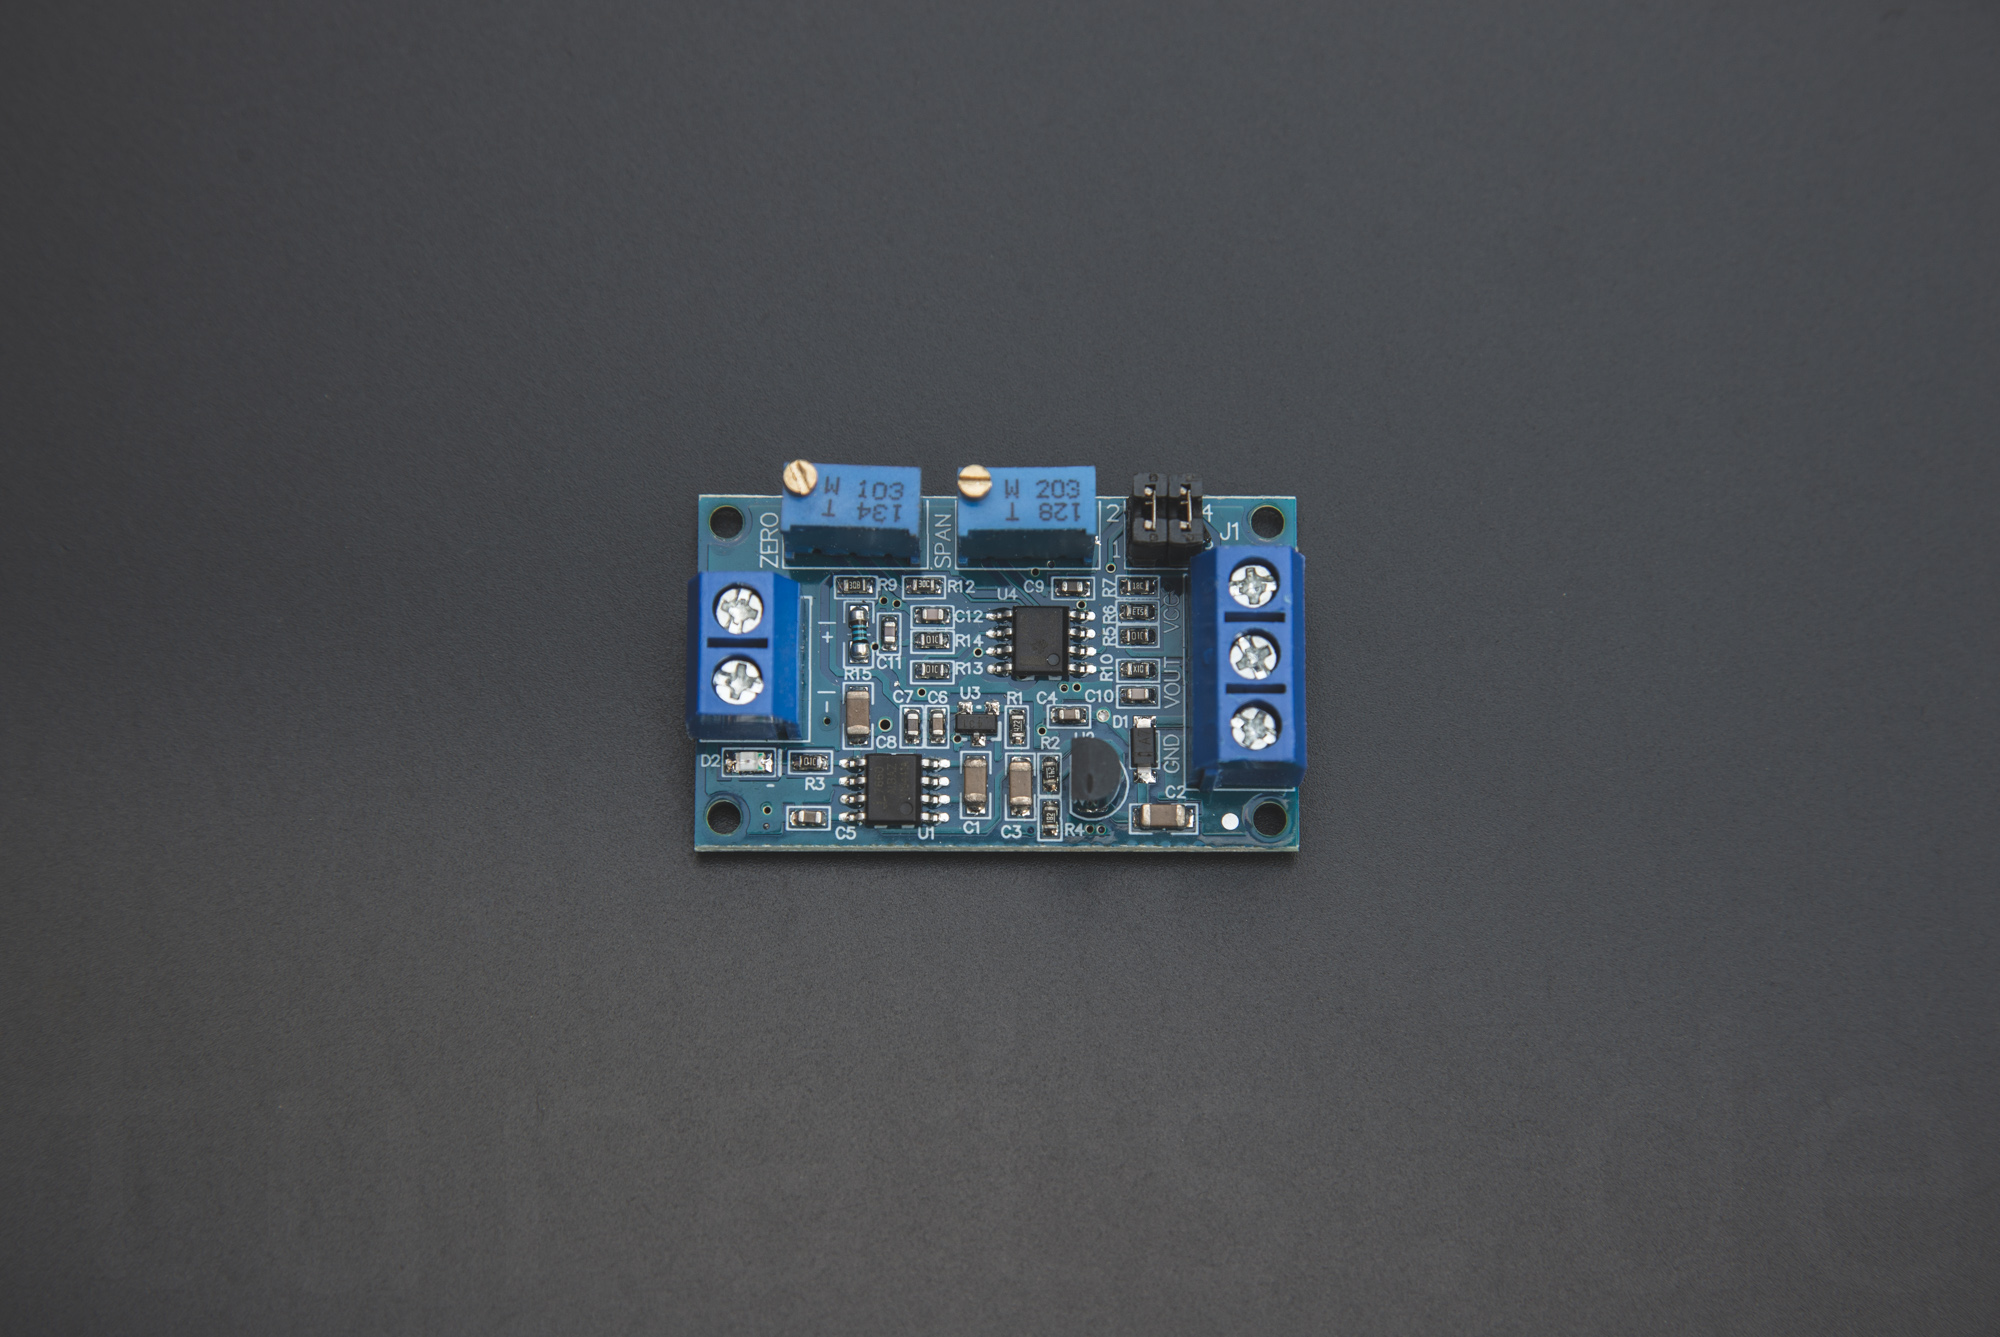
\includegraphics[width=\linewidth]{graphics/strom_sensor_modul.jpg}
        \caption{HW-685 Amperage to Voltage converter}
    \end{subfigure}
    \caption{Components used during hardware assembly}
    \label{fig:hardware-setup}
\end{figure}

The Raspberry Pi hosts the software components responsible for data processing, storage, and visualization. All hardware components are powered by using appropriate DC voltage levels, and special care and professional advice was taken to ensure electrical separation and safe wiring between the circuits.

\begin{figure}[H]
    \centering
    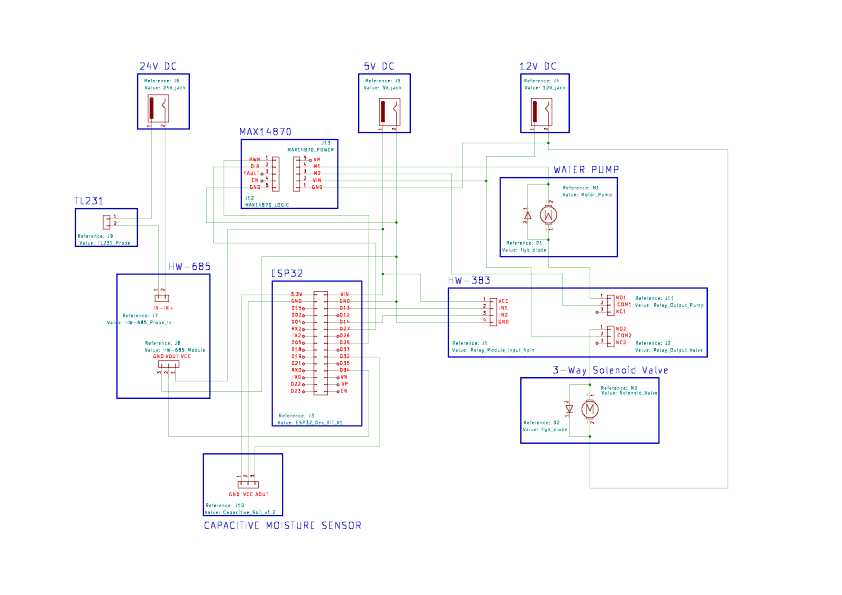
\includegraphics[width=1\textwidth]{ oasis-schematic-v3.png}
    \caption{Schematics of the hardware}
    \label{fig:placeholder}
\end{figure}



\subsection{Software Structure}

The software architecture of OASIS is divided into distributed components running on the ESP32 and the Raspberry Pi. 

The ESP32 firmware is responsible for reading the sensor data, performing the basic preprocessing and publishing the measurements to the MQTT Broker. It also subscribes to the control topics to receive irrigation commands and actuates the pump accordingly.

The Raspberry Pi runs multiple software services. A Python based control application subscribes to MQTT topics to receive soil moisture data and acts as the central decision logic of the system. Incoming sensor data is stored in InfluxDB, a local time-series database optimized for sensor measurements.

For visualization purposes, Grafana is used to query InfluxDB and display soil moisture data and system behavior in interactive dashboards. In addition, the Raspberry Pi integrates the WeatherAPI to retrieve historical rainfall data, which is used to make even better decisions.

\begin{figure}[H]
    \centering
    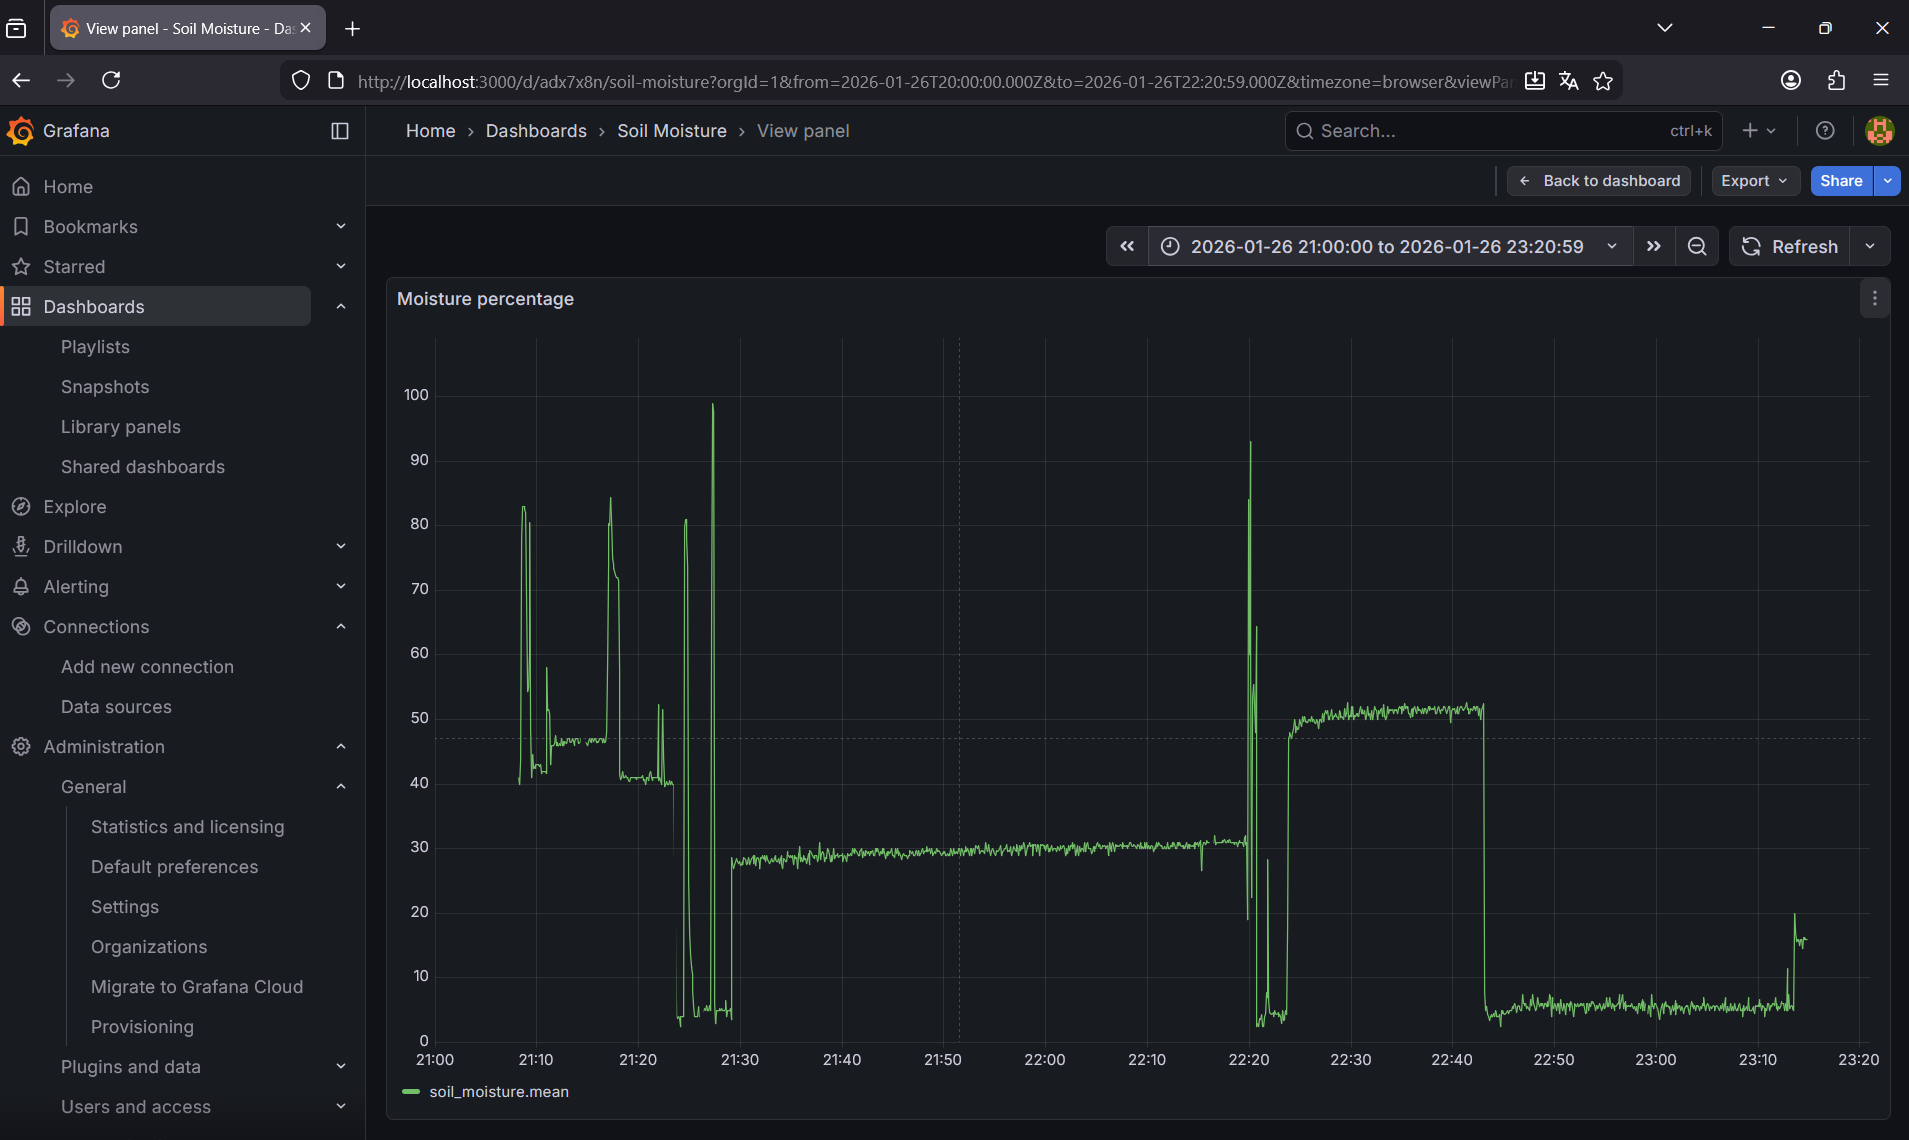
\includegraphics[width=0.75\linewidth]{graphics/Grafana-Soil_Measure.png}
    \caption{Visualization of Soil Measurements using Grafana}
    \label{fig:placeholder}
\end{figure}

\begin{figure}[H]
    \centering
    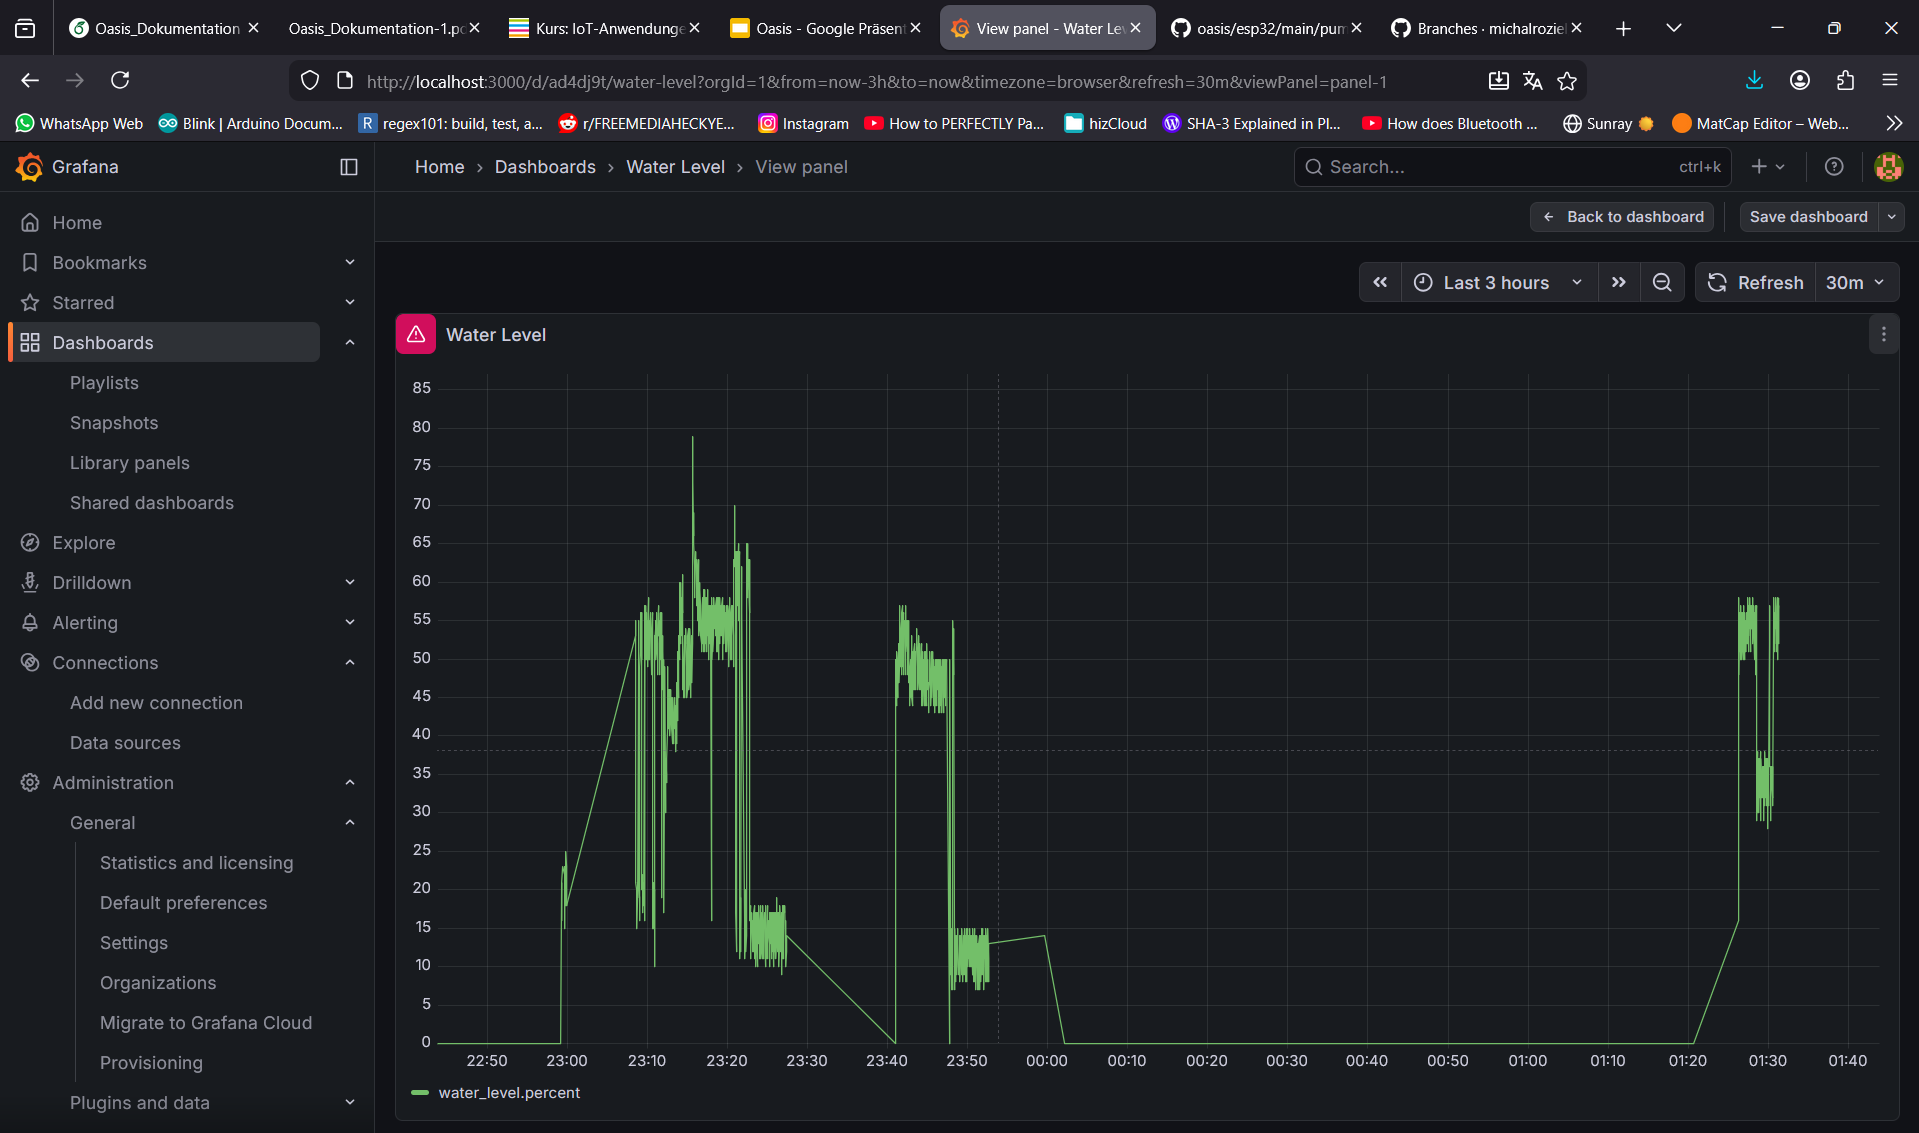
\includegraphics[width=0.75\linewidth]{graphics/Water_Level_Sensor.png}
    \caption{Visualization of Water Tank Level using Grafana}
    \label{fig:placeholder}
\end{figure}


\subsection{Communication and Data Flow}
Communication between the system components is realized using a combination of MQTT and HTTPS interfaces. The ESP32 publishes soil moisture measurements to predefined MQTT topics via a public HiveMQ broker. The Raspberry Pi subscribes to these topics and receives data asynchronously. 

After receiving the data, the raspberry Pi stores the measurements in InfluxDB and retrieves the historical rainfall information from the WeatherAPI using HTTPS requests. Based on the combination of soil moisture and recent rainfall data, the control logic decides whether irrigation is permitted or not.

If watering is allowed, the Raspberry Pi publishes a corresponding control command to the MQTT broker. The ESP32, which subscribes to this control topic, receives the command and activates or deactivates  the water pump accordingly.

InfluxDB acts as a passive data storage component and does not actively send data to any modules. Grafana queries InfluxDB at configurable intervals to retrieve the saved data for visualization. This pull-based approach ensures a clear separation between data storage, processing and visualization.  


\section{Build and Setup Guide}

\subsection{Bill of Materials}
\begin{table}[H]
    \centering
    \footnotesize
    \begin{tabularx}{\textwidth}{|l|X|c|l|c|}
    
    \hline
        \textbf{Name} & \textbf{Usage} & \textbf{Quantity} & \textbf{Acquired By} & \textbf{Cost(€)}\\
    \hline
        Large Project Enclosure & Project Case & 1 & Micha{\l} & 15 \\
    \hline
        Small Project Enclosure & Project Case & 1 & Micha{\l} & 10 \\
    \hline
        11L water tank & Water saving tank & 1 & Micha{\l} & 19 \\
    \hline
        3L water tank & Simulation of rainwater & 1 & Micha{\l} & 10 \\
    \hline
       Phoenix contact terminal blocks & Safe Distribution of DC Voltages & 6 & Micha{\l} & Pre-Owned \\
    \hline
        mounting rails  & mounting of terminal blocks & 1 & Micha{\l} & Pre-Owned \\
    \hline
       mounting screws  & mounting of sensors \& base plates & 20 & Micha{\l} & Pre-Owned \\
    \hline
        Water valve & actuating the rainwater & 1 & Micha{\l} & 3 \\
    \hline
        ESP32 Breadboard Kit & Bits and Pieces & 1 & Micha{\l} & 23 \\
    \hline
       DC jack connectors & Power supply to the project & 1 & Micha{\l} & 8 \\
    \hline
       Custom wooden base plate & mounting base for sensors \& rails & 2 & Micha{\l} & Created \\
    \hline
       TL231 & 24V DC water pressure sensor & 1 &EmRoLab  & Given \\
    \hline
       HW-685 & 5V DC Voltage-Amperage Converter & 1 & EmRoLab & Given \\  
    \hline
       Capacitive moisture sensor v1.2 & Soil moisture monitoring & 1 & EmRoLab & Given \\  
    \hline
       12V DC water Pump  & pumping water from water tank to plants & 1 & EmRoLab & Given \\  
    \hline
       12V DC Solenoid Valve  & 3-Way diverter to either tank or drain & 1 & Micha{\l} & 15 \\  
    \hline
       230V Relay  & Used to relay Voltage to Pump and Solenoid Valve & 2 & EmRoLab & Given \\  
    \hline
       5V DC Power Supply & Supply Power to Esp and Relays & 1 & Micha{\l} & Pre-Owned \\  
    \hline
       12V DC Power Supply & Supply Power to Pump and Solenoid Valve & 1 & EmRoLab & Given \\  
    \hline
       24V DC Power Supply & Supply Power to TL231 & 1 & EmRoLab & Given \\
    \hline
    \end{tabularx}
    
    \caption{Bill of Materials}  
    \label{tab:bom}
\end{table}


\subsection{Wiring and Assembly}
The wiring and assembly of the OASIS System were carried out in a modular and safe manner. Due to the use of multiple DC voltage levels (5V , 12V, 24V), Phoenix contact terminal blocks were employed to ensure a clear separation of power domains and reliable distribution of supply voltages.

All components were mounted inside custom wooden base plates. The ESP32 and low-voltage controls were provided with 5V of power, while the water pump and the valve operated at 12V. The pressure sensor required a separate 24V supply. Relays were used to isolate the low-voltage control logic from the higher voltage loads. 

Special Care was also taken to route signal wires and power cables separately to reduce interference.  All connections were tested for correct polarity and secure mounting before powering the system.


\subsection{Firmware Upload}
The ESP32 firmware was developed using the Arduino IDE. Prior to uploading the firmware, the ESP32 was connected to a host computer via USB. The correct board type and serial port were selected in the development environment. 

Configuration parameters such as WiFi credentials and MQTT information were defined before flashing the firmware. After uploading, the serial monitor was used continuously to verify the connection to the network and the publication of the data.

\subsection{Initial Startup and Commissioning}
During initial startup, the system was powered on step by step to ensure the correct operation of all components. First, the Raspberry Pi and database services wer started and verified. Next the ESP32 was powered and observed via the serial monitor. 

Sensor readings were checked for plausibility and relay switching was done and  tested by Micha{\l} to verify correct pump and valve control. Once all components behaved as expected, the water system was activated and the full irrigation system workflow was tested under controlled conditions.

\subsection{Troubleshooting}
Several challenges were encountered during development and testing. Network connectivity issues occasionally occurred due to incorrect  WiFi credentials and restricted networks.

Incorrect sensor readings were addressed by recalibrating the soil moisture sensor and checking the wired connections. Actuators, relays and power supply voltages were checked over and over again during the development process.





\section{Work Distribution (Group Work)}
\subsection{Roles and Responsibilities}
All software components of the project were developed by using the Git-Repostory made by \emph{Micha{\l}}:  \url{https://github.com/michalroziel/oasis}. The repository was used to manage source code, config files and documentation throughout the development process. 

Each contributor worked on dedicated features and components and had his own responsibilities and tools, which can be seen in the table below: 


\begin{table}[H]
    \centering
    \begin{tabular}{|l|p{6cm}|p{5cm}|c|}
    \hline
         \textbf{Team Member} & \textbf{Responsibilities} & \textbf{Tools} & \textbf{Effort}  \\
         \hline
         Hanan & Software Implementation and Documentation & Raspberry Pi, Grafana, InfluxDB, Latex  & 65 \\
         \hline
         Micha{\l} & Hardware and Software Implementation, Documentation  & Power Tools, Sensors, Electrical circuits, Latex  & 110 \\
         \hline
         Laith & Software Implementation & Raspberry Pi and Python Scripts & 65 \\
         \hline
         Omar & Software Implementation & Raspberry Pi and Python Scripts & 65 \\
         \hline
    \end{tabular}
    \caption{Task Distribution und Effort}
    \label{tab:placeholder}
\end{table}

\subsection{Individual Contributions}
Here, each team members individual contributions are presented. The respective contributions reflect their share of the total workload.

\subsubsection{Omar Qoul}
Contributed to the development of the ESP32 firmware, including the implementation and calibration of sensor readings. Additionally, I assisted with the configuration of InfluxDB and contributed to the implementation of the WeatherAPI, which supported decision-making related to irrigation control. Played a vital role in the testing of MQTT connections and was responsible for the presentations alongside Laith.

\subsubsection{Laith Arafeh}
Calibrated the soil-moisture sensor and tested the water level sensor used to monitor the rainwater tank. Helped in writing the Firmware for the ESP32 that reads, converts, and transmits the sensor values from the ESP32 to the MQTT broker. 
Set up the MQTT infrastructure and configured the HiveMQ broker and is responsible for the presentations alongside Omar.


\subsubsection{Hanan Ahmed Ashir}
Responsible for the Software implementation of the project. Installed and configured InfluxDB and Grafana on the raspberry Pi, managed sensor data, integrated Grafana for time-series visualization, and incorporated the WeatherAPI to enable more logical decisions alongside Omar and Laith. In addition, responsible for authoring the complete project documentation and coordinating the distribution of tasks among the team members.

\subsubsection{Micha{\l} Roziel}

Picked up the hardware components which the \textit{EmRoLab} team provided us with. Bought and provided additional hardware components listed in the bill of materials. Created custom wooden base plates for both hardware enclosures by using power as well as precision (woodworking) tools.
Drilled holes into both project enclosures to fit previously mentioned base plates and self soldered DC-Jack connectors. Connected all of the wiring found in the project. Tested, connected, assembled and installed all of the hardware used in the project.
Sensor testing was done by using a high fidelity Fluke multimeter.
Contributed to the establishing of communication between the ESP32 and Raspberry Pi via MQTT. 

Created In-depth project schematic showcasing internal logic and electrical connections.\\
Contributed to all project presentations throughout the course. Contributed to collaborative project documentation using \LaTeX.

\section{Outlook and Lessons Learned}

\subsection{Future Improvements}

As a future improvement, the system could be deployed on a remote server instead of running exclusively on a local Raspberry Pi. This would enable remote access to sensor data and system status, increase scalability and allow the project to be maintained as an open source solution. By publishing the data other users and developers could reuse and extend the system for their own applications.

Additional improvements could include the integration of further environmental sensors and use of weather forecasts in addition to the historical rainfall data to further optimize irrigation decisions.

\subsection{Lessons Learned}

\begin{itemize}

    \item A major challange during hardware assembly was the integration of components operating at different voltage levels. The water sensor required 24V, while the ESP32 is limited to 5V. To ensure safe operation, relays, Phoenix Contact Terminal blocks and different amperage to voltage converters were used to isolate the high voltage circuit. Overcoming this challenge improved the team's understanding of mixed voltage system design.

    \item Furthermore, implementing communication between the ESP32 and the raspberry Pi using the MQTT publish/subscribe model significantly improved the teams understanding of system architecture.
    
    \item A practical limitation that we encountered during the project was related to the network accessibility. Since Grafana and InfluxDB were configured to run on the raspberryPi using localhost bindings, access to the dashboard was only possible within the local network. As a result, connections via public or university WiFi networks were not feasible without additional configuration, for which we had little to no time.

    \item Another problem encountered was the sensitivity of the water level sensor provided to us\emph{Figure 2(a)}. Since the sensor is designed to handle huge tanks, the smaller tank that we had handled severe fluctuations, hereby preventing us from getting any stable readings\emph{(Figure 5)}. To solve this, we hard coded the diverter to move the water around based on the Raspberry Pi's decisions.
\end{itemize}

\section{References}
This section provides an overview of the references and supporting materials used throughout the development of the project. During the implementation, various external sources were consulted to ensure correct technical decisions and proper system design. In addition, images were taken during the development process to support the explanation of the system. 

\subsection{Images}
\begin{figure}[H]
    \centering
    
    \begin{subfigure}[b]{0.45\textwidth}
        \centering
        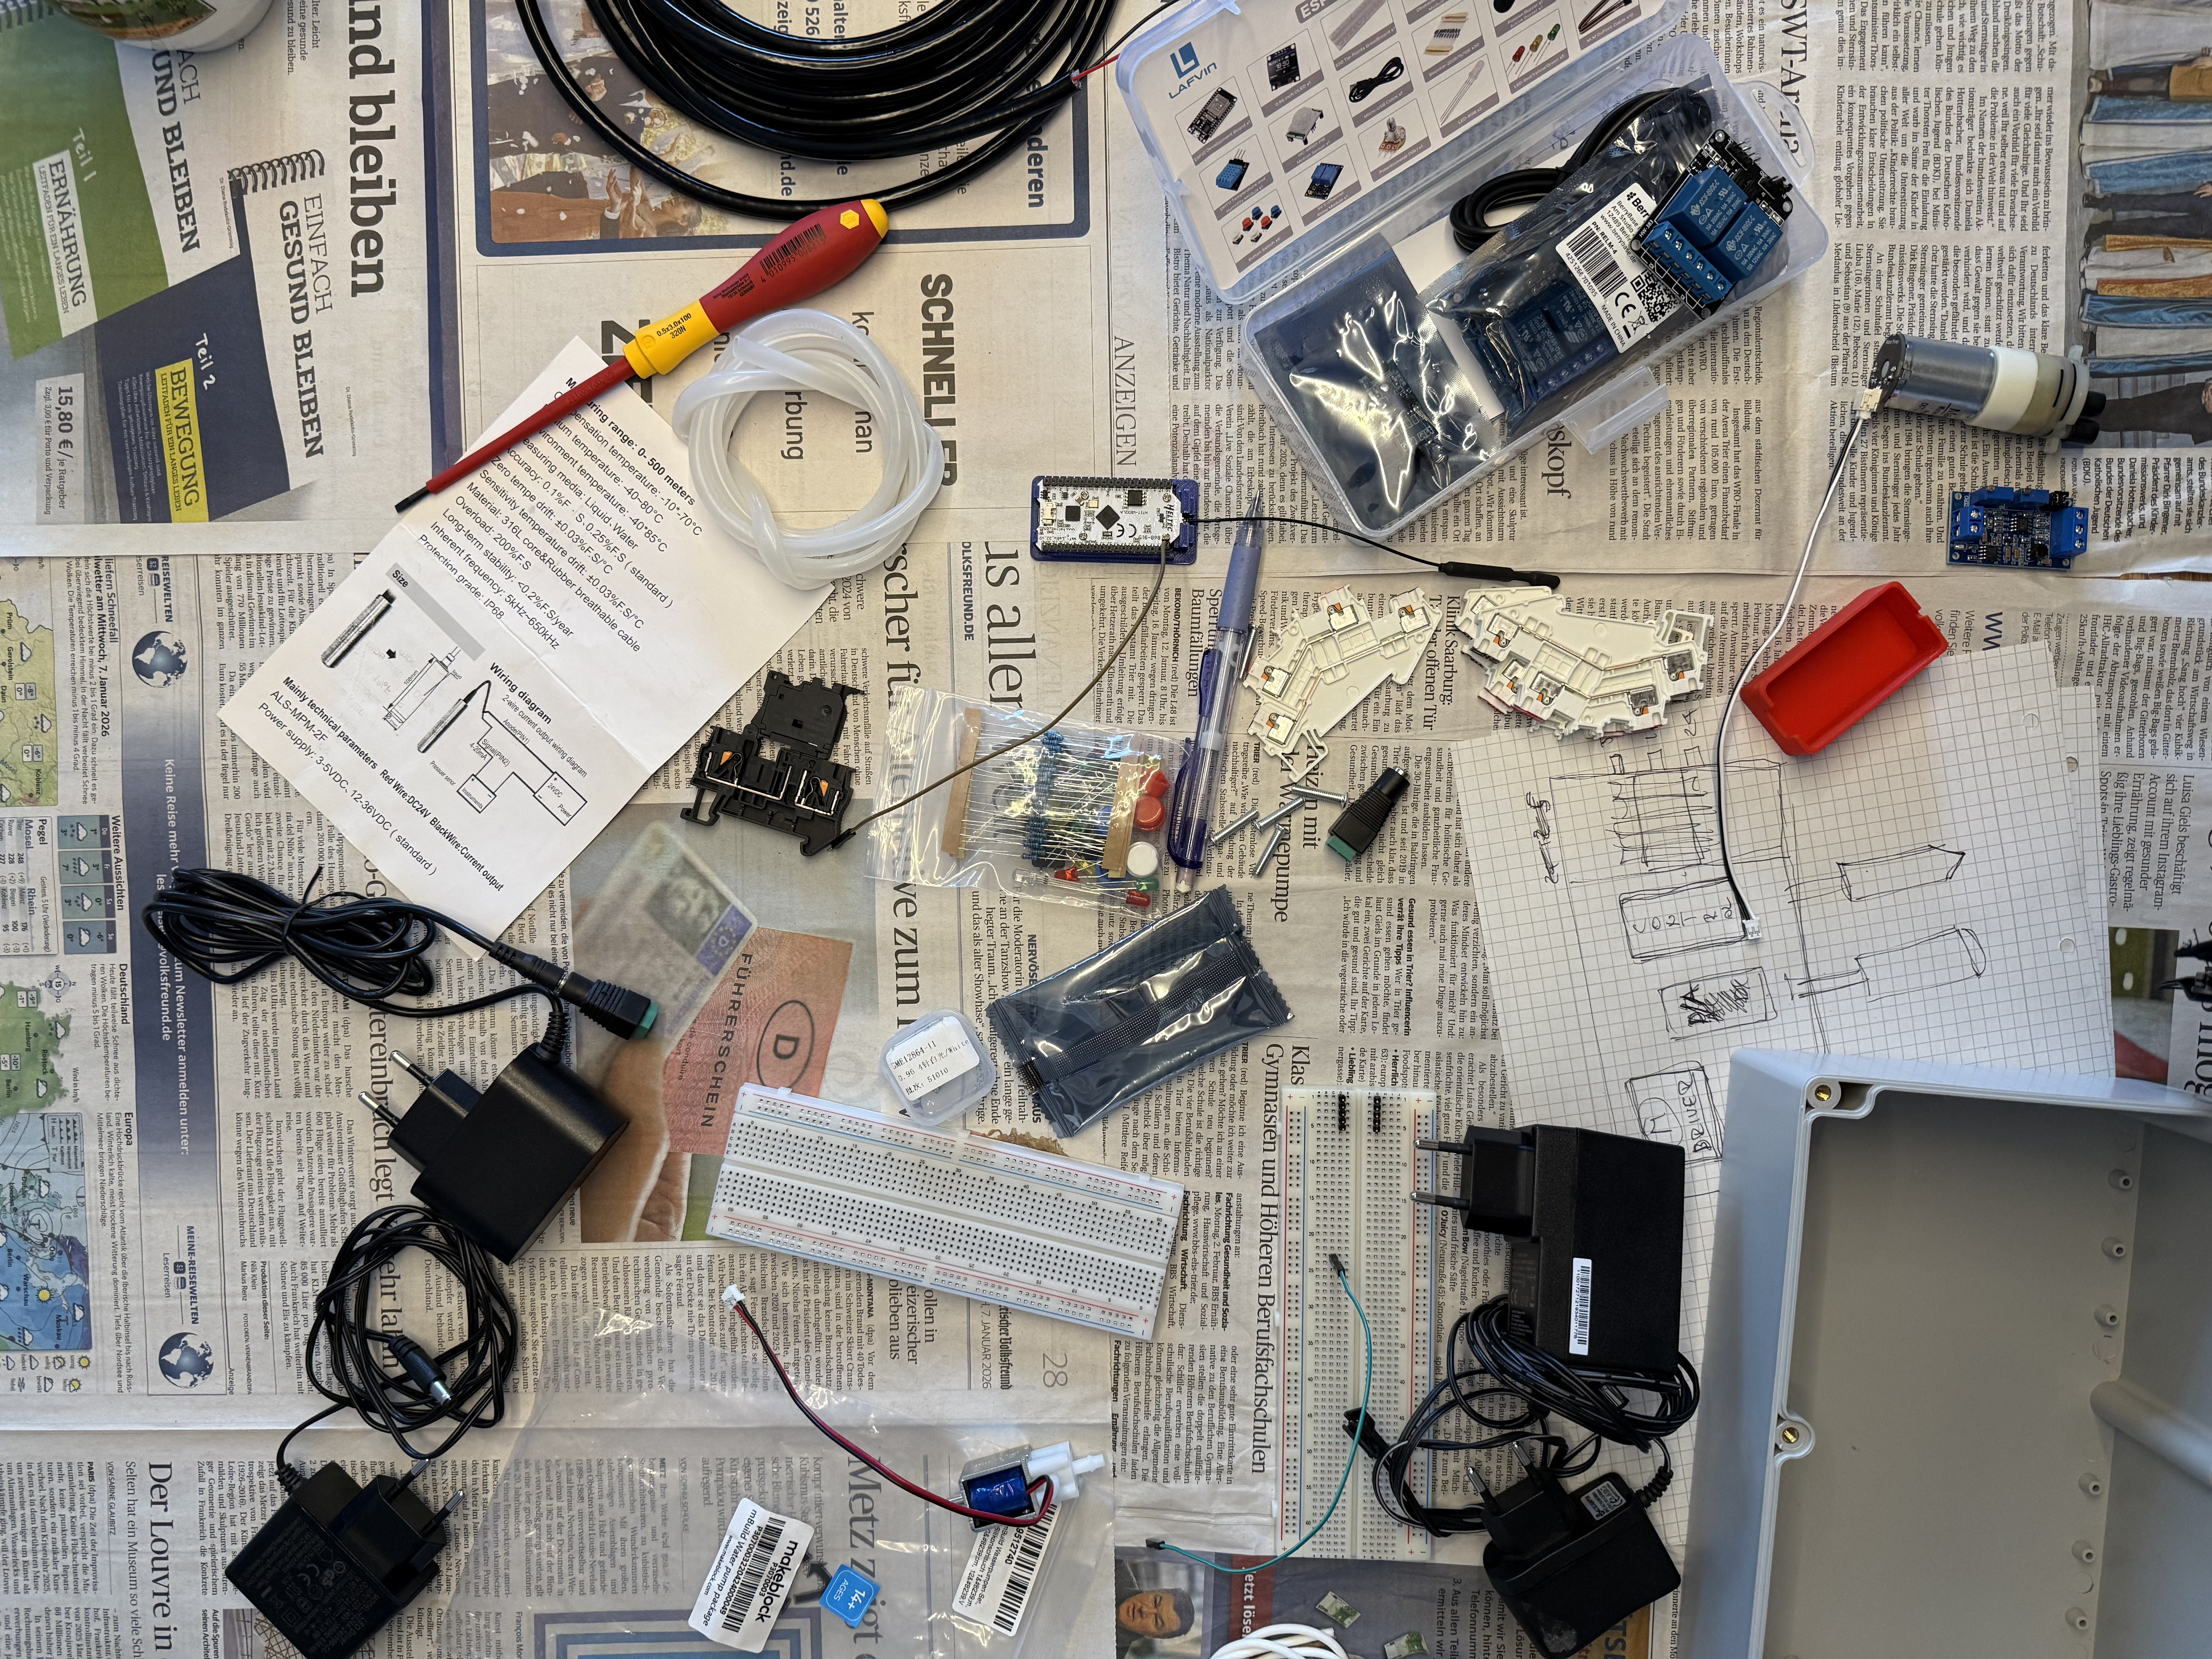
\includegraphics[width=\textwidth, height=8cm, keepaspectratio]{graphics/dev-1.jpeg} 
        \caption{Start of assembly}
        \label{fig:assembly_1}
    \end{subfigure}
    \hfill
    \begin{subfigure}[b]{0.45\textwidth}
        \centering
        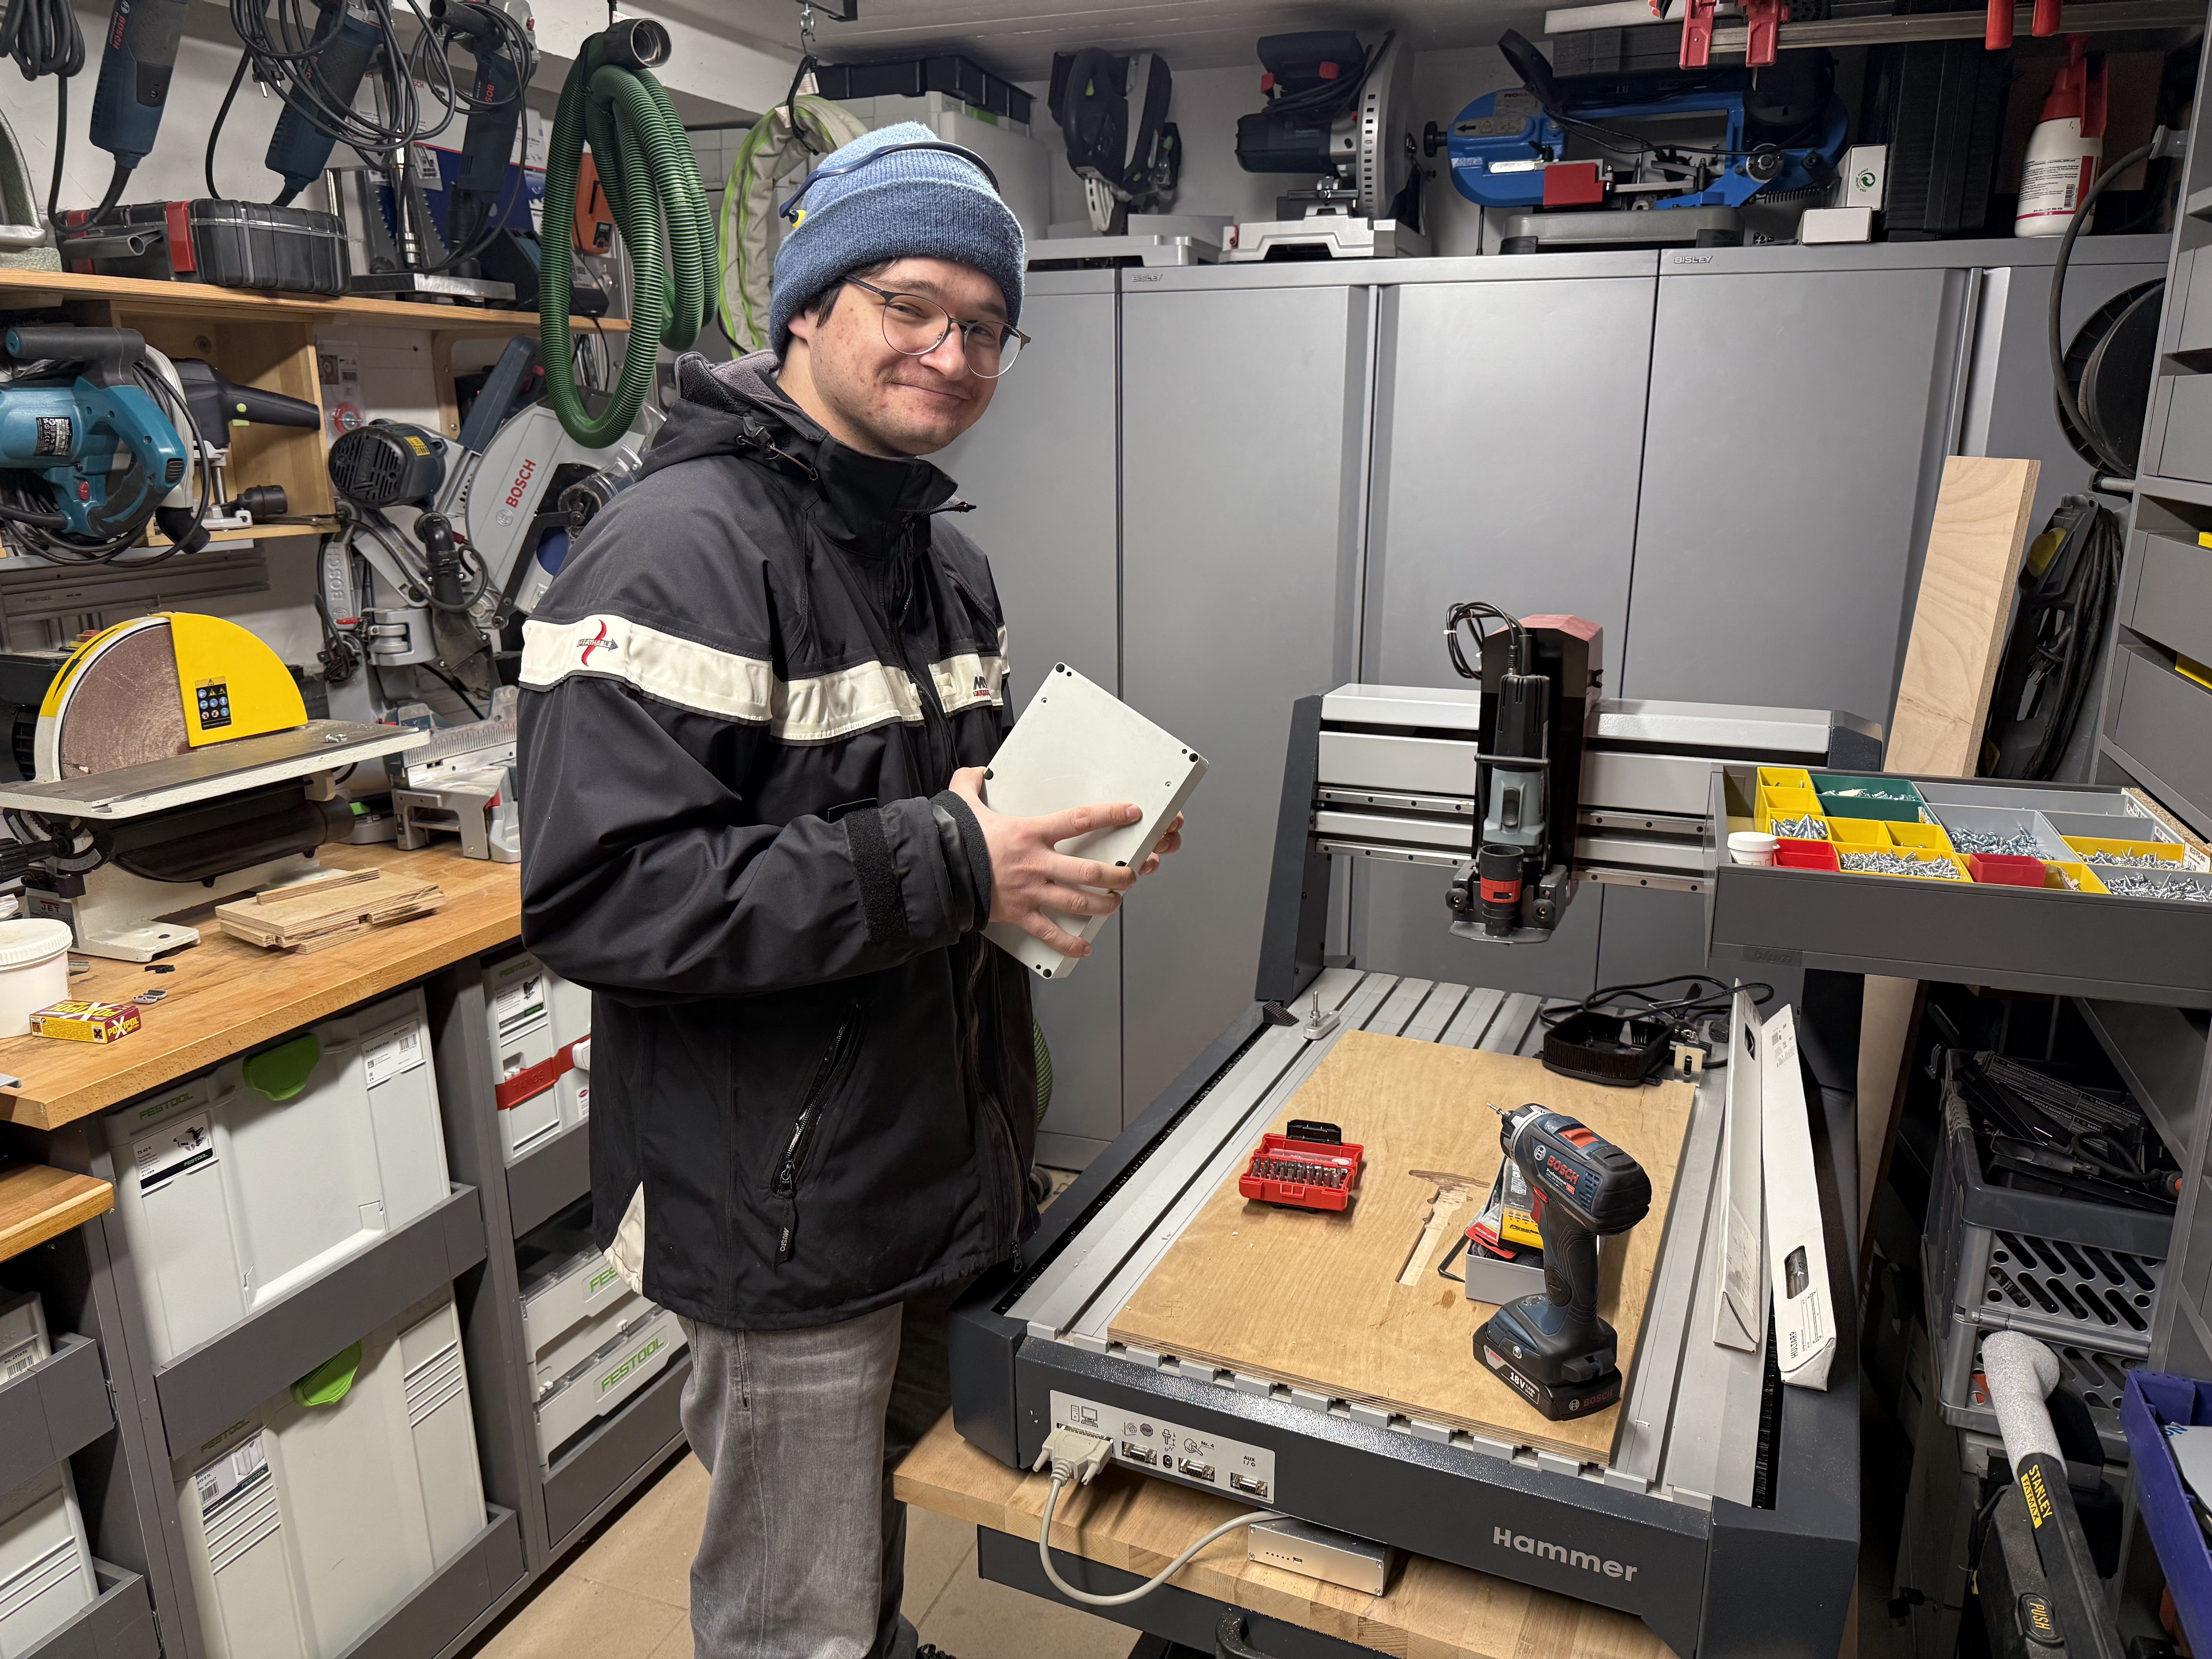
\includegraphics[width=\textwidth, height=8cm, keepaspectratio]{graphics/dev-2.jpeg}
        \caption{In the workshop}
        \label{fig:assembly_2}
    \end{subfigure}
    
    \vspace{1cm} % Space between rows

    \begin{subfigure}[b]{0.45\textwidth}
        \centering
        % Added keepaspectratio so rotation doesn't distort image
        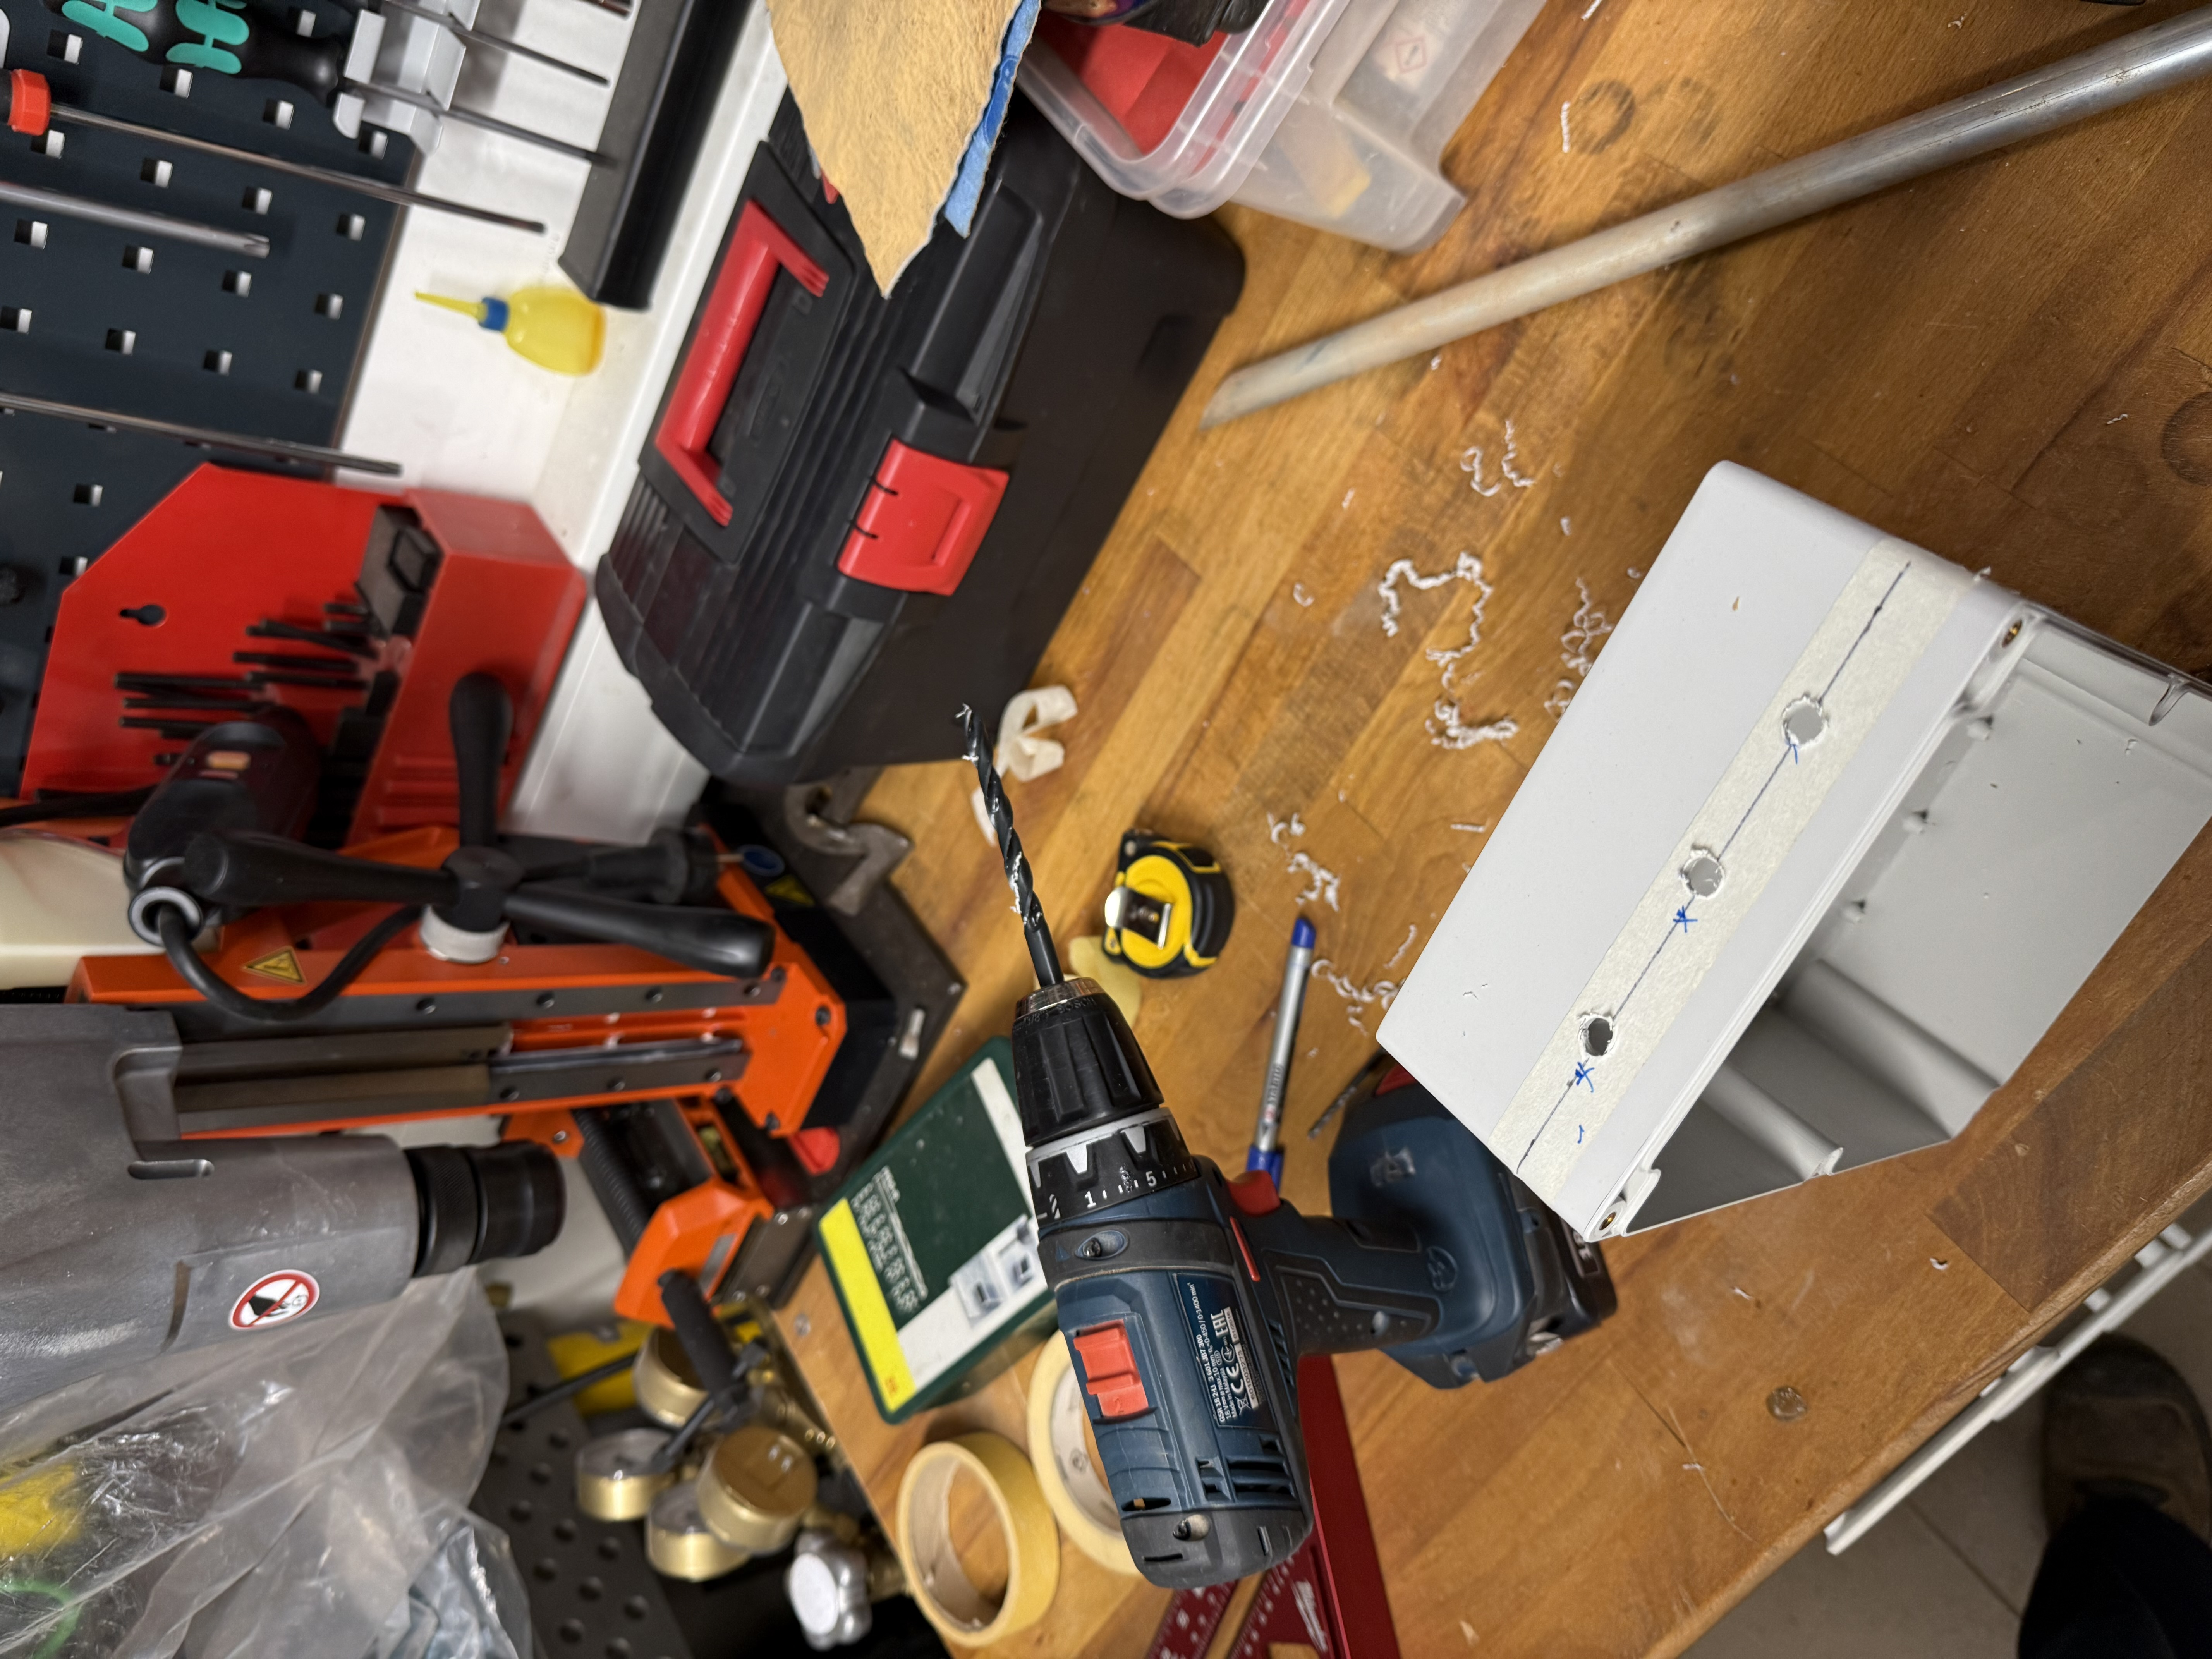
\includegraphics[width=\textwidth, height=8cm, angle=270, keepaspectratio]{graphics/dev-10.jpeg}
        \caption{Drilling holes into enclosure}
        \label{fig:assembly_3}
    \end{subfigure}
    \hfill 
    \begin{subfigure}[b]{0.45\textwidth}
        \centering
        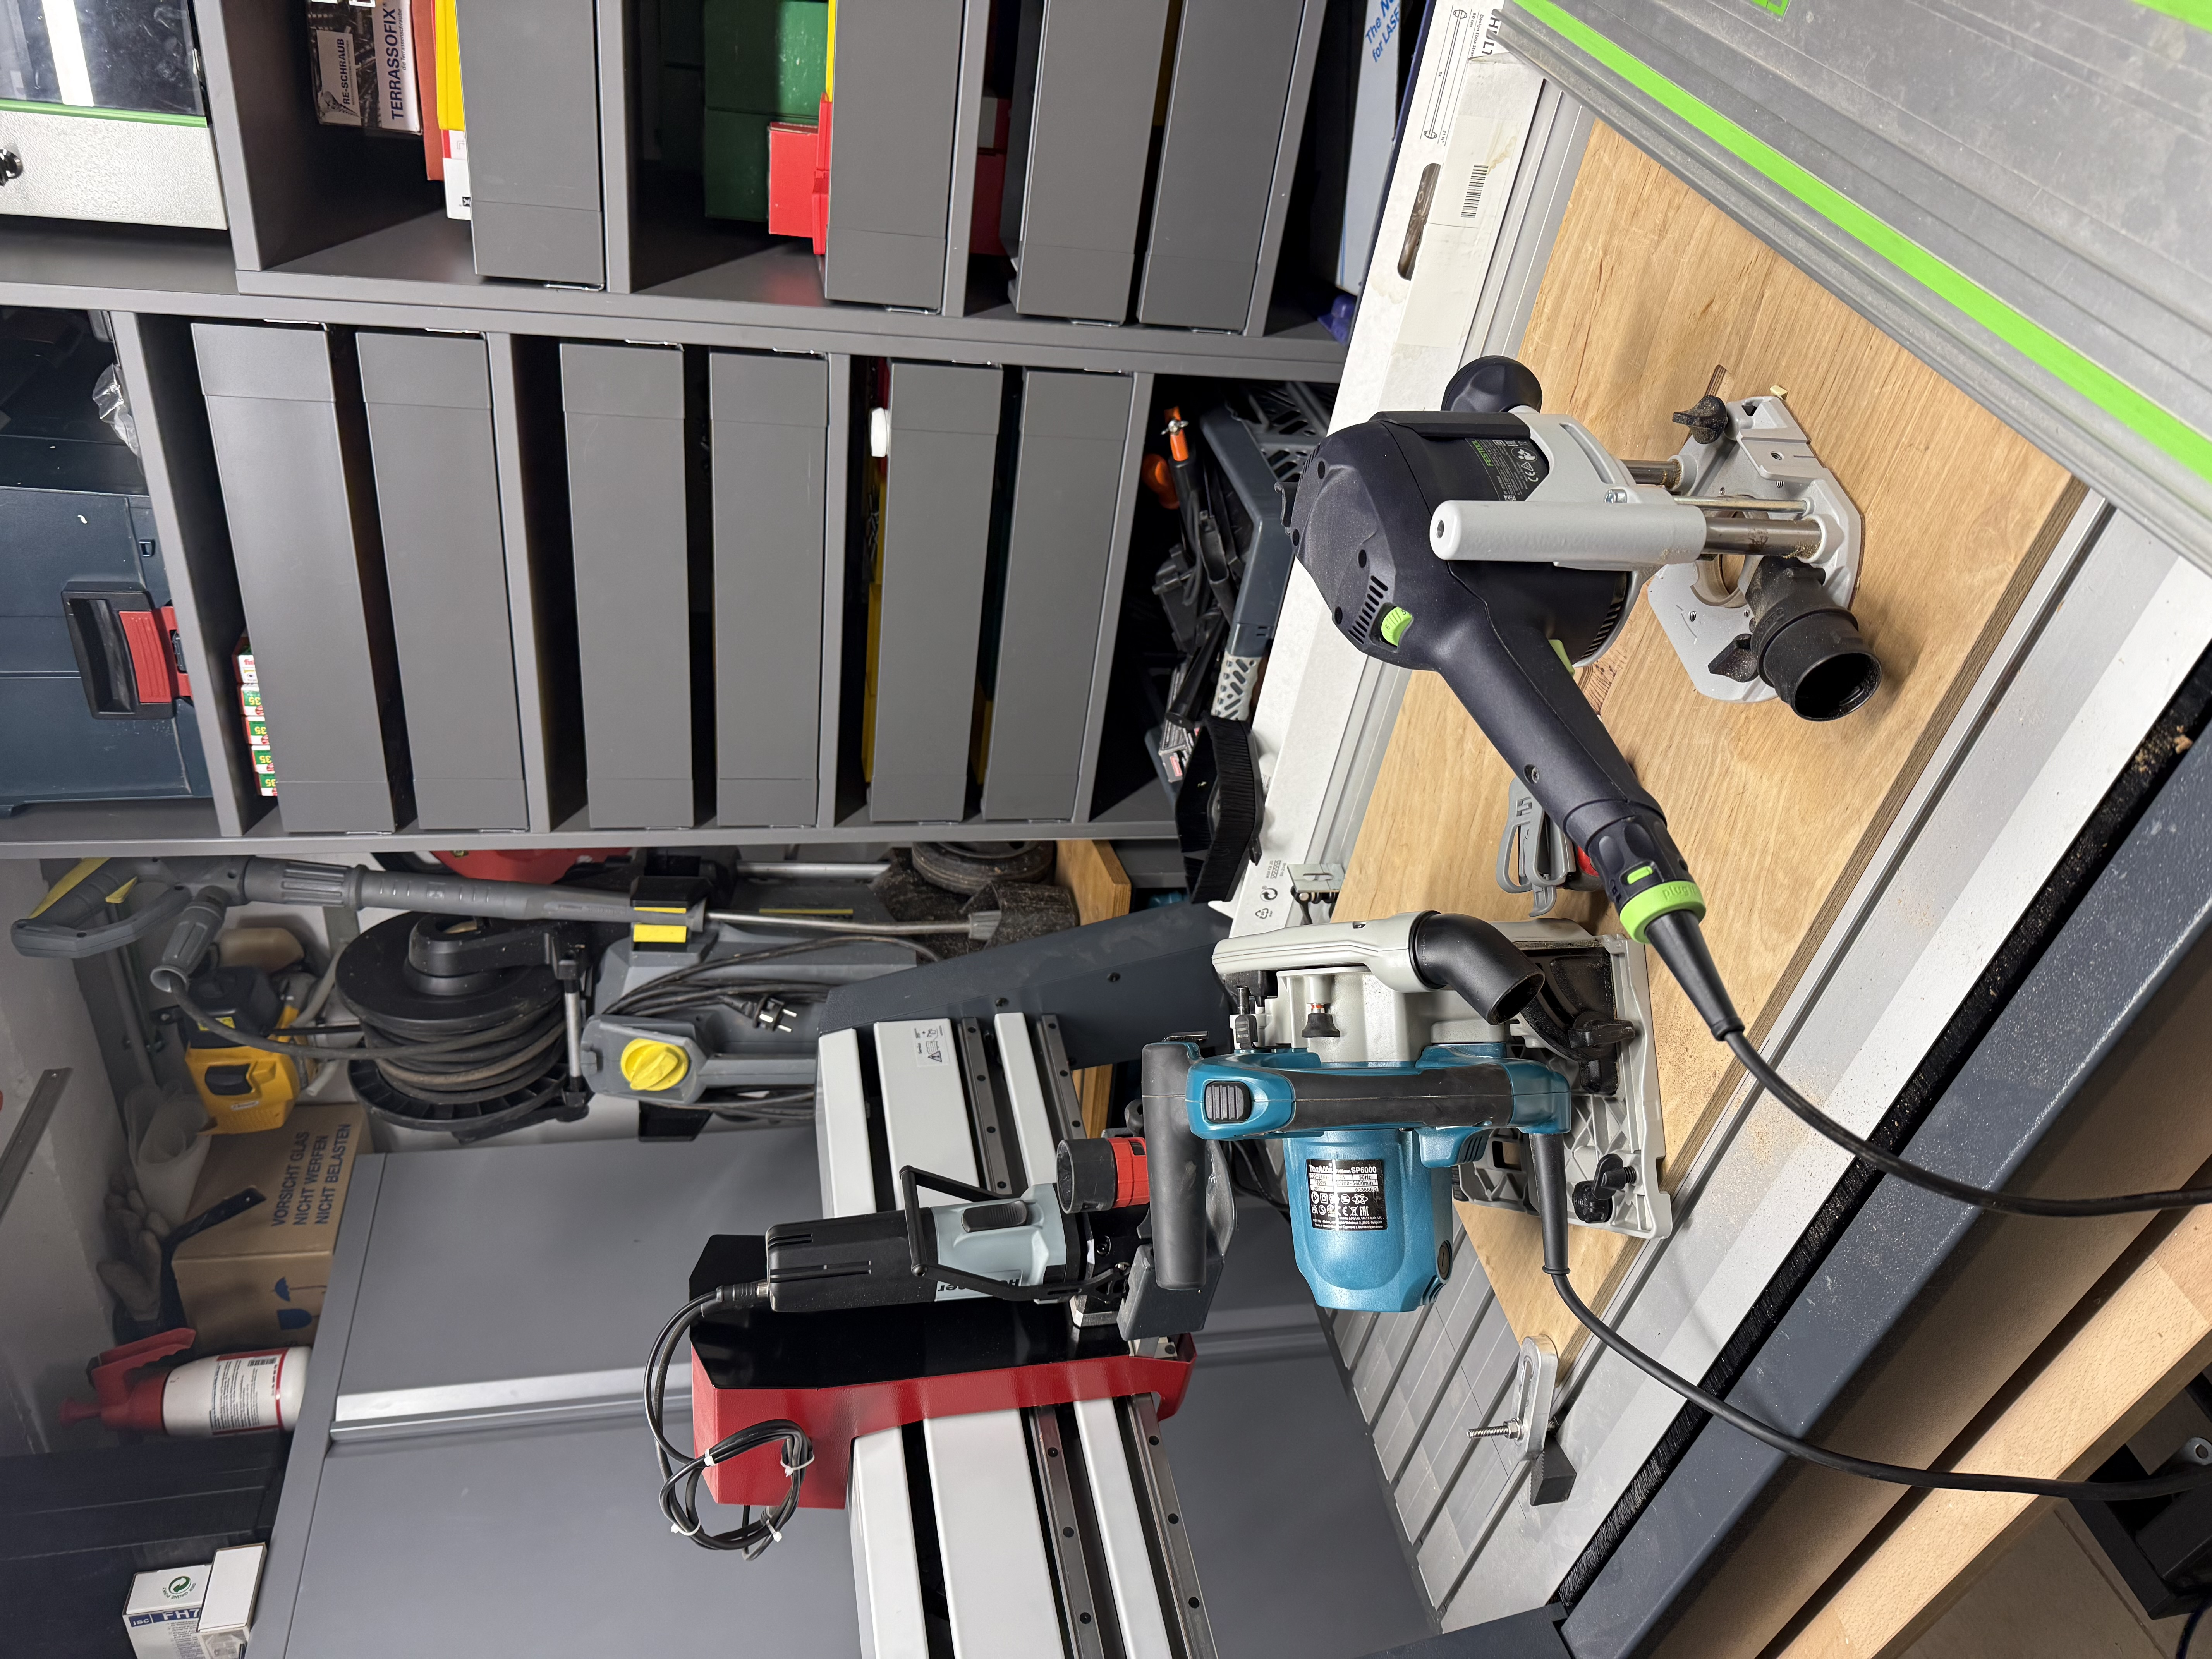
\includegraphics[width=\textwidth, height=8cm, angle=270, keepaspectratio]{graphics/dev-9.jpeg}
        \caption{Wooden enclosure baseplate }
        \label{fig:assembly_4}
    \end{subfigure}

    \vspace{1cm} 

    \caption{Hardware Assembly Process (Part 1)}
    \label{fig:gallery_page1}
\end{figure}

\clearpage % Forces a page break for the next set of images

% --- REPEAT THE BLOCK ABOVE FOR PAGE 2 ---

\clearpage % Forces a page break so the gallery starts on a fresh page

\begin{figure}[p] % [p] tells LaTeX "Put this on a dedicated page only for figures"
    \centering
    
    % --- ROW 1 ---
    \begin{subfigure}[b]{0.45\textwidth}
        \centering
        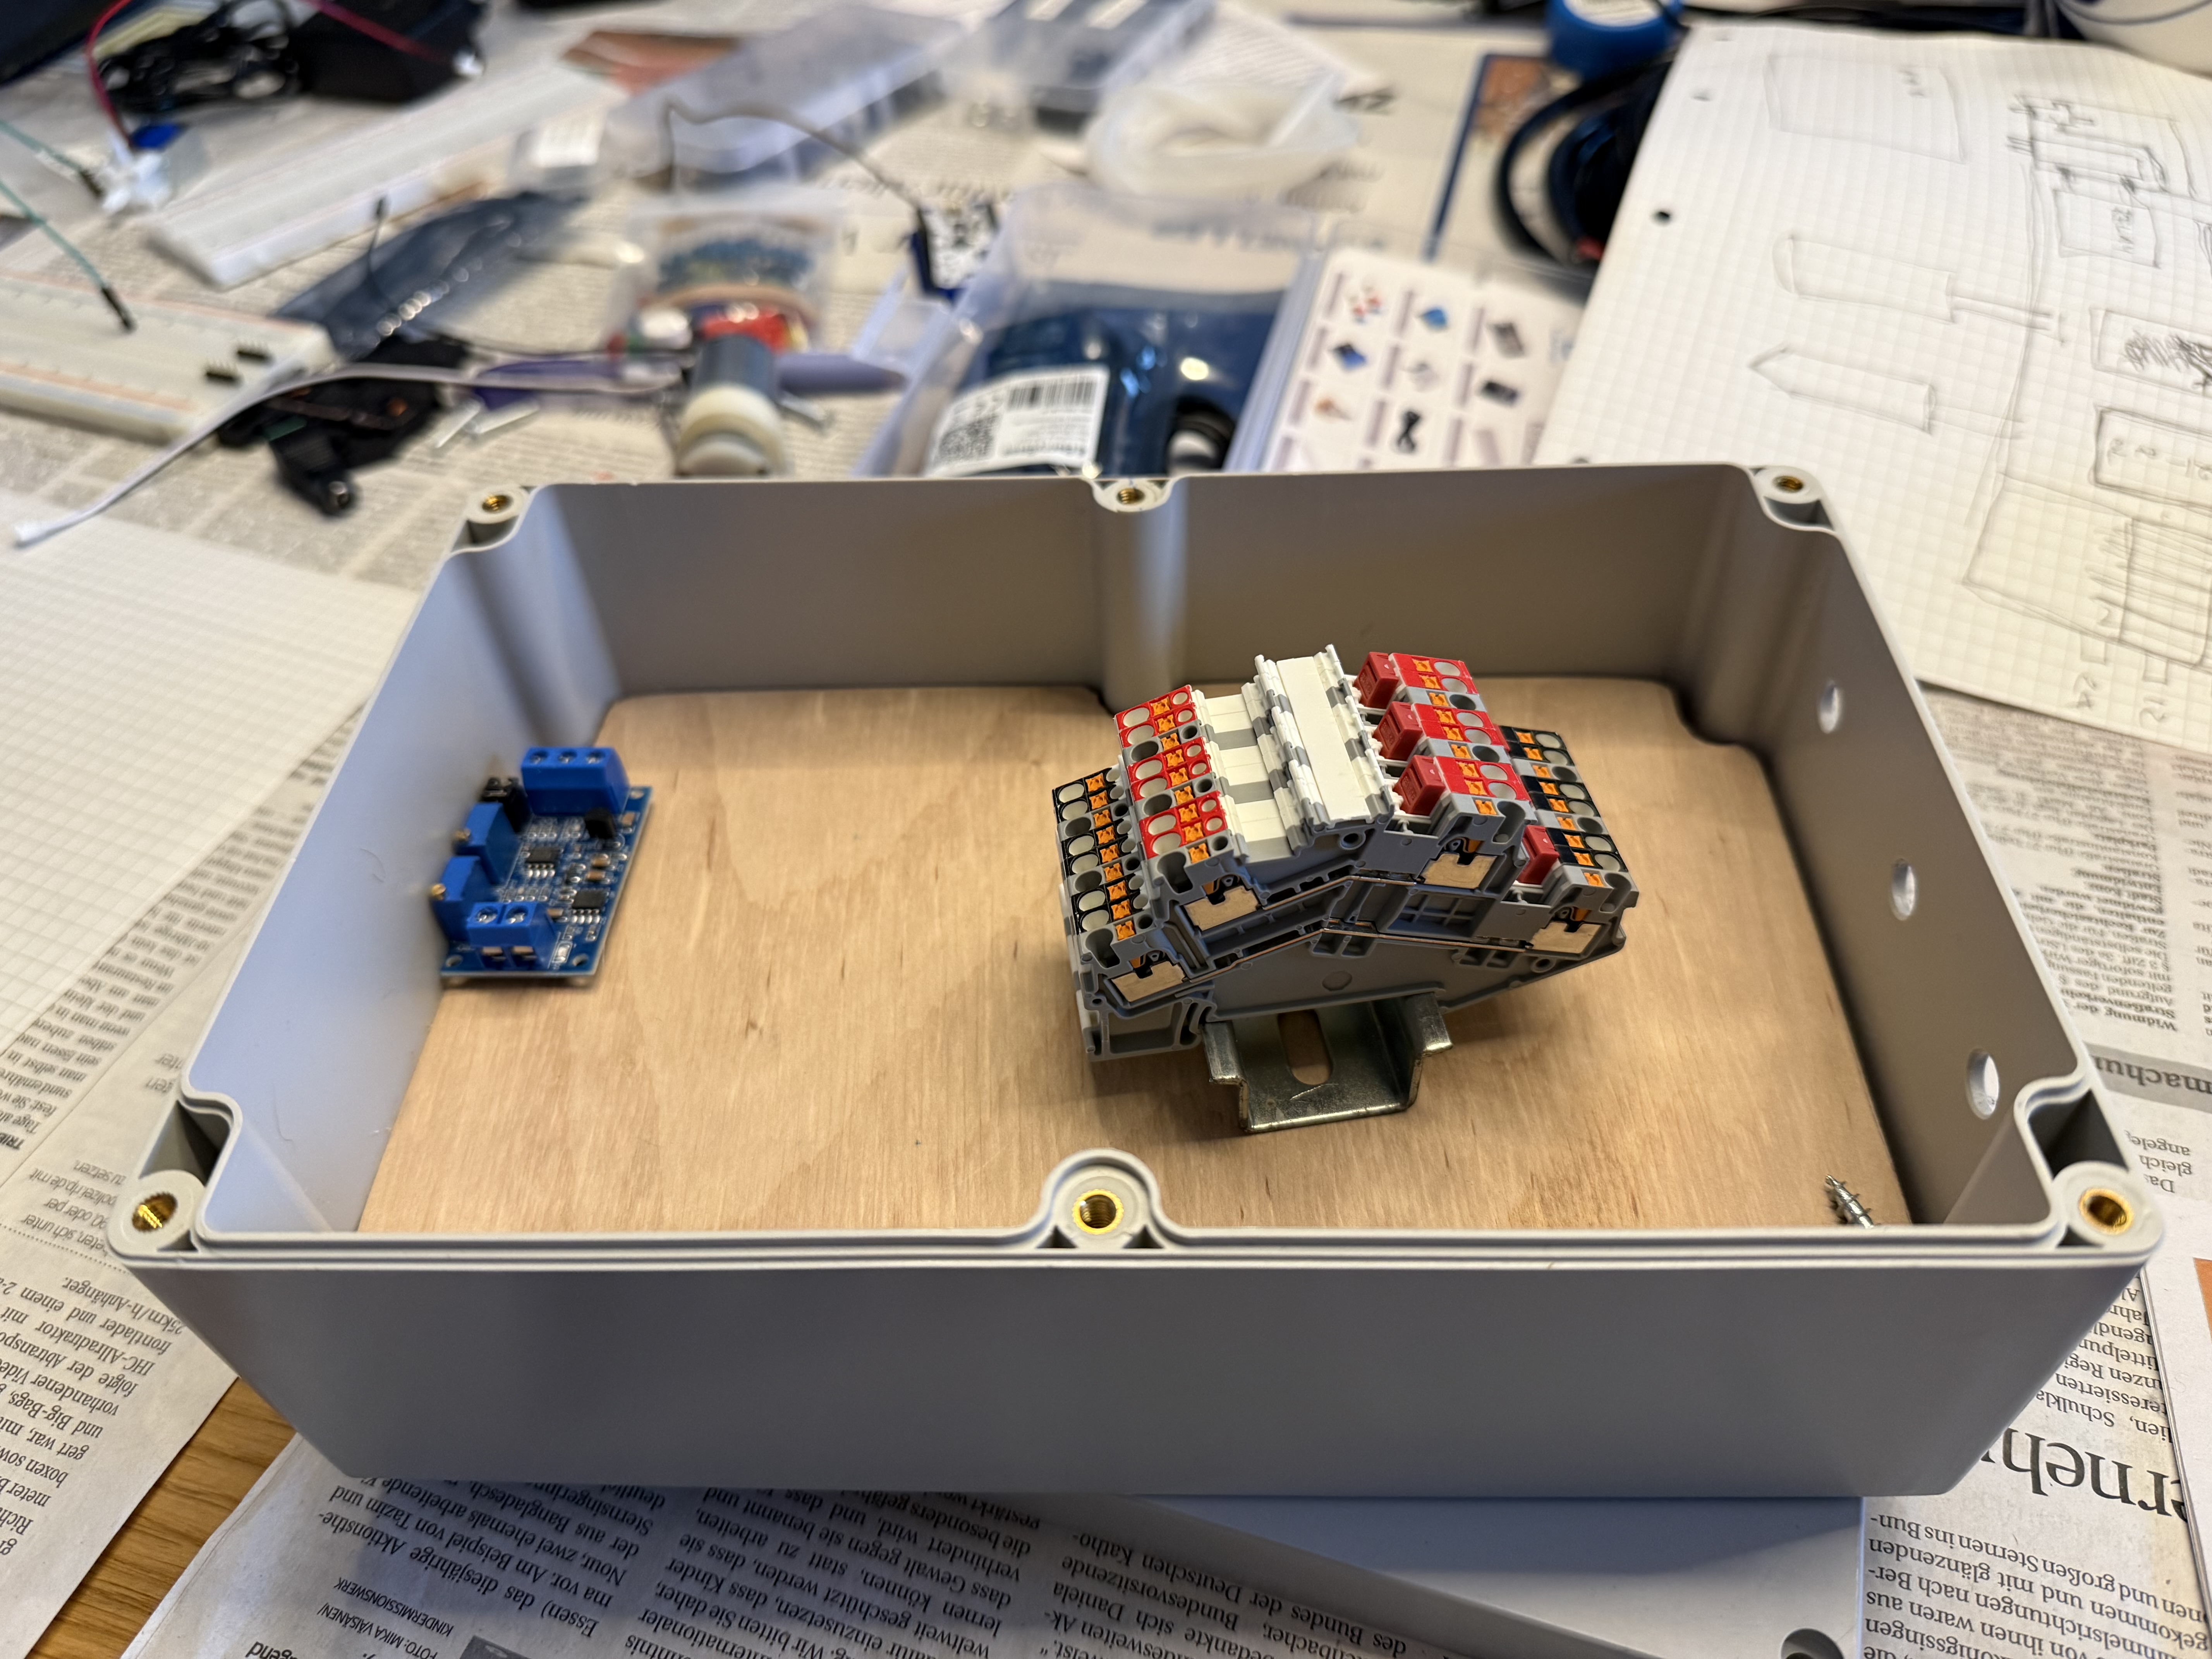
\includegraphics[width=\textwidth, height=5cm, keepaspectratio]{graphics/dev-4.jpeg} 
        \caption{mounting terminal blocks}
        \label{fig:assembly_1}
    \end{subfigure}
    \hfill % Pushes images apart
    \begin{subfigure}[b]{0.45\textwidth}
        \centering
        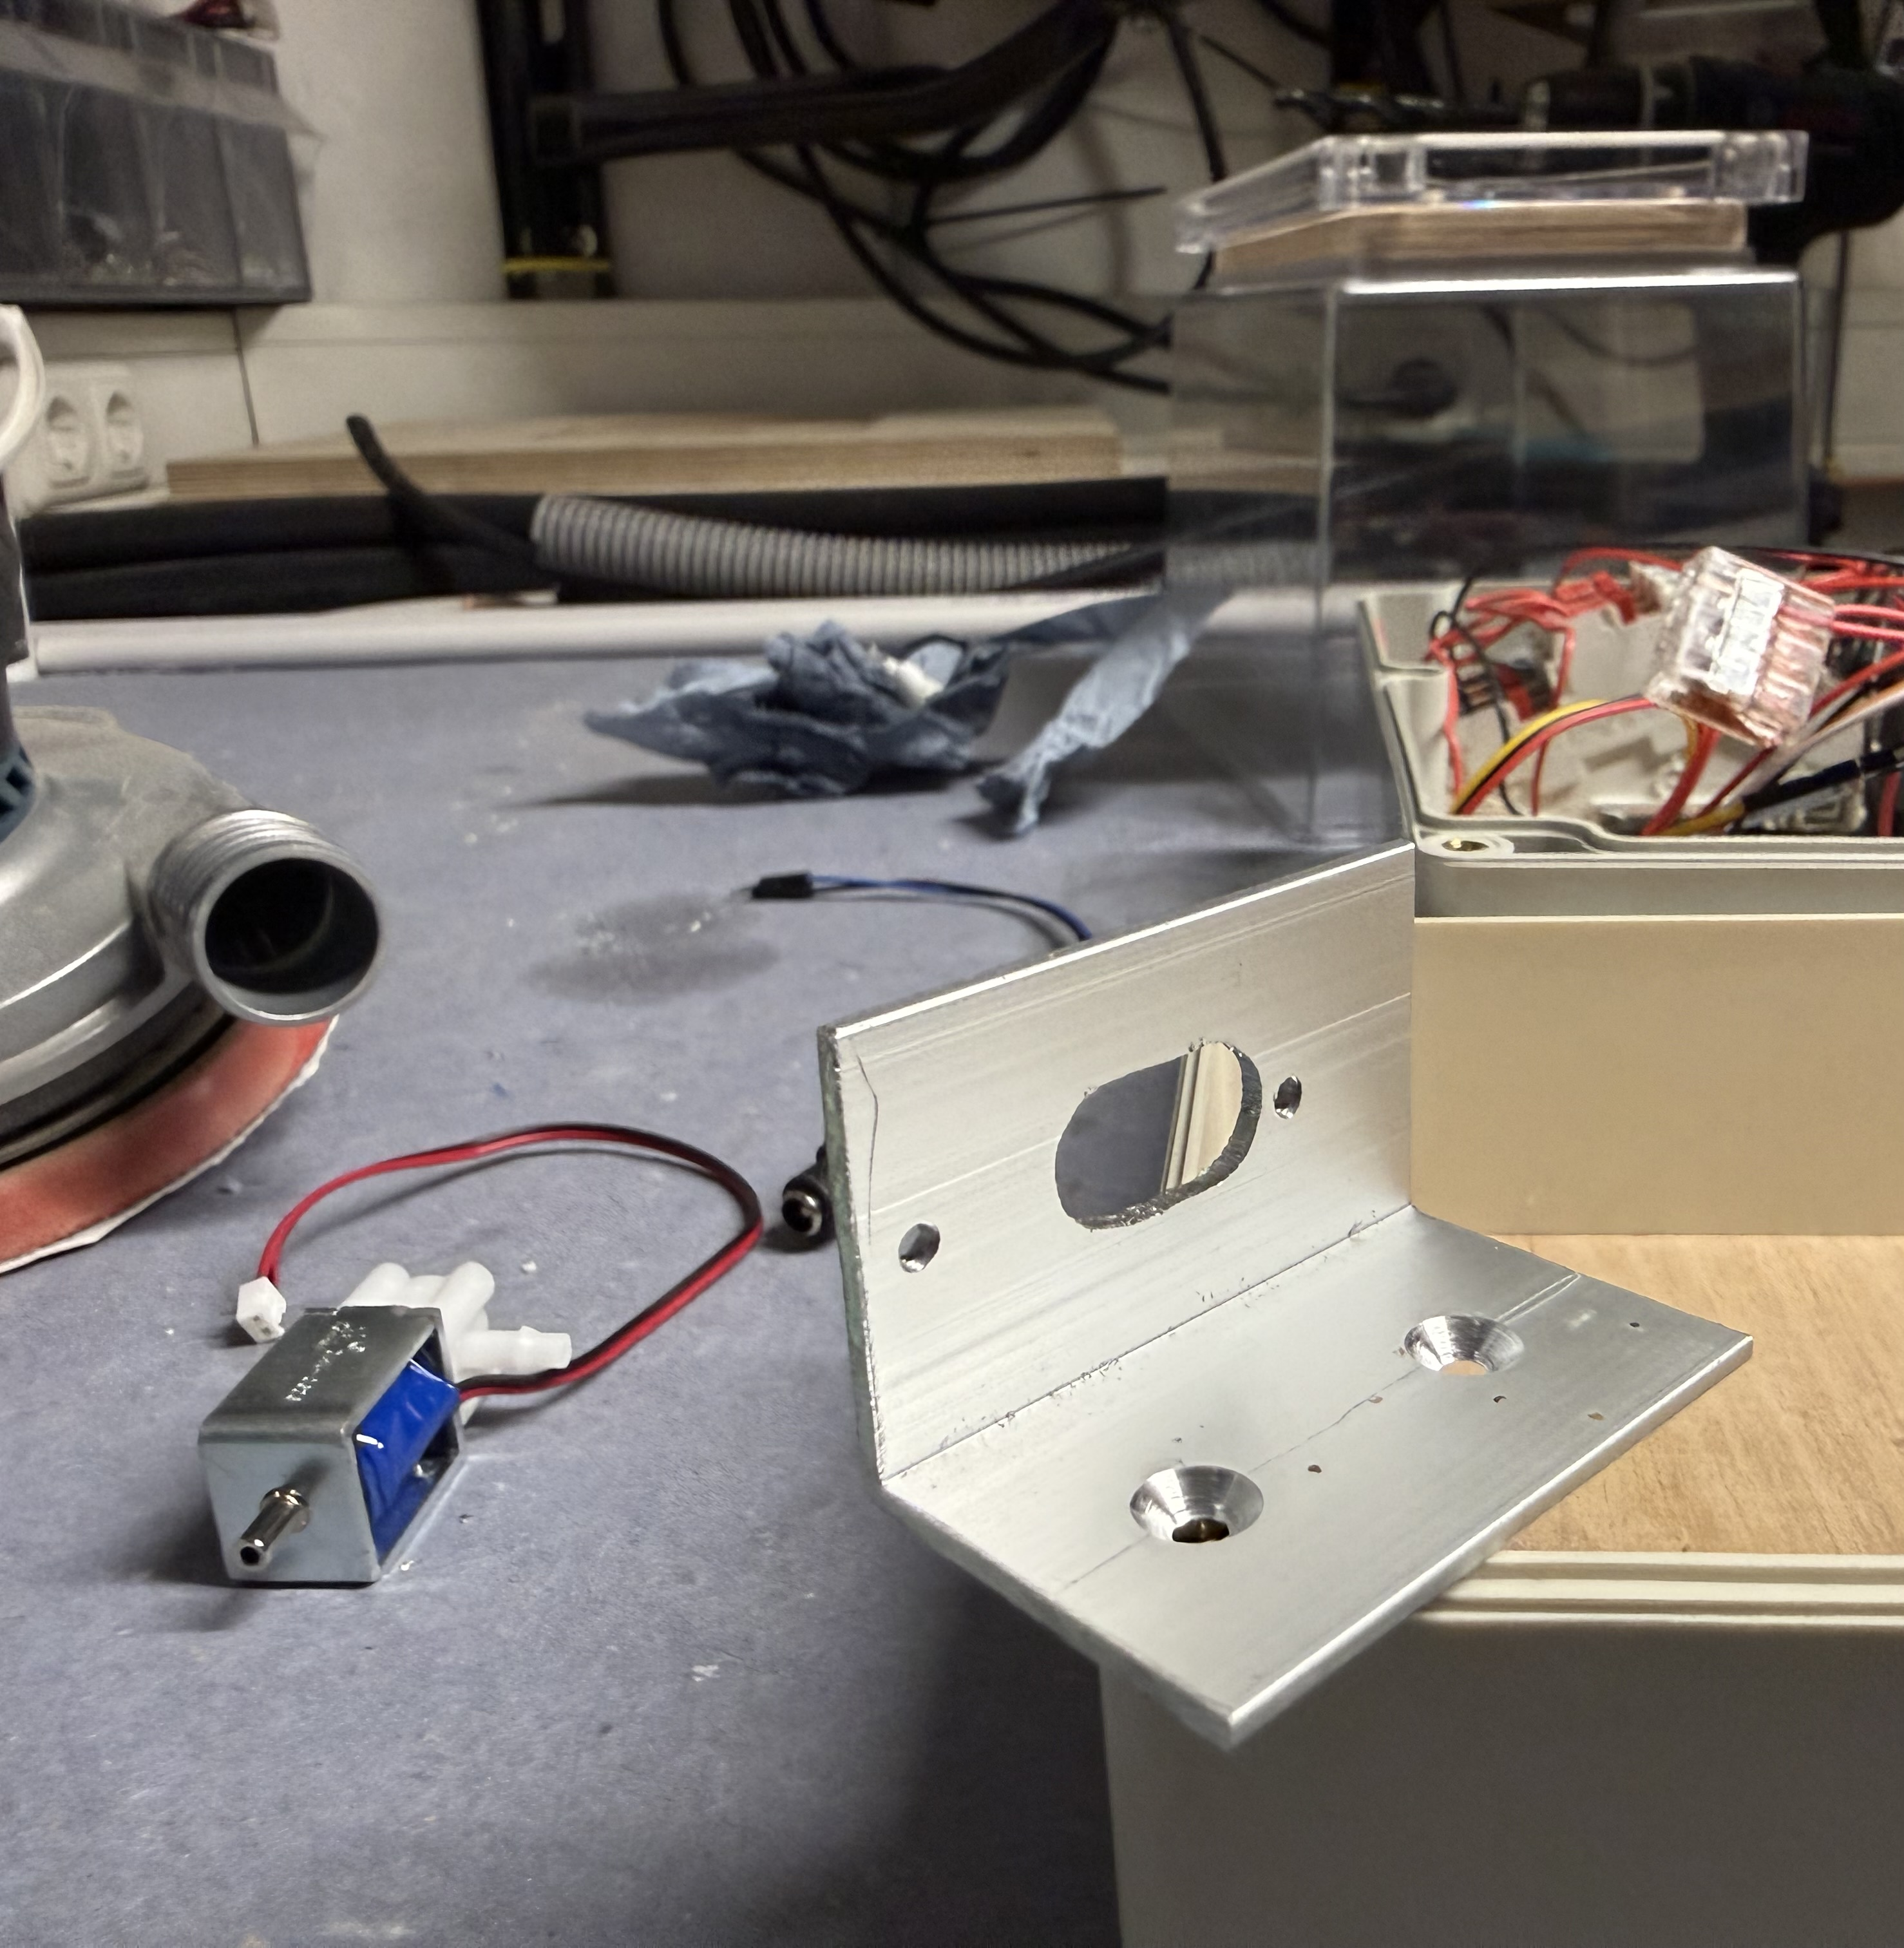
\includegraphics[width=\textwidth, height=5cm, keepaspectratio]{graphics/dev-8.jpeg}
        \caption{aluminum mounting plate}
        \label{fig:assembly_2}
    \end{subfigure}
    
    \vspace{1cm} % Vertical space between rows

    % --- ROW 2 ---
    \begin{subfigure}[b]{0.45\textwidth}
        \centering
        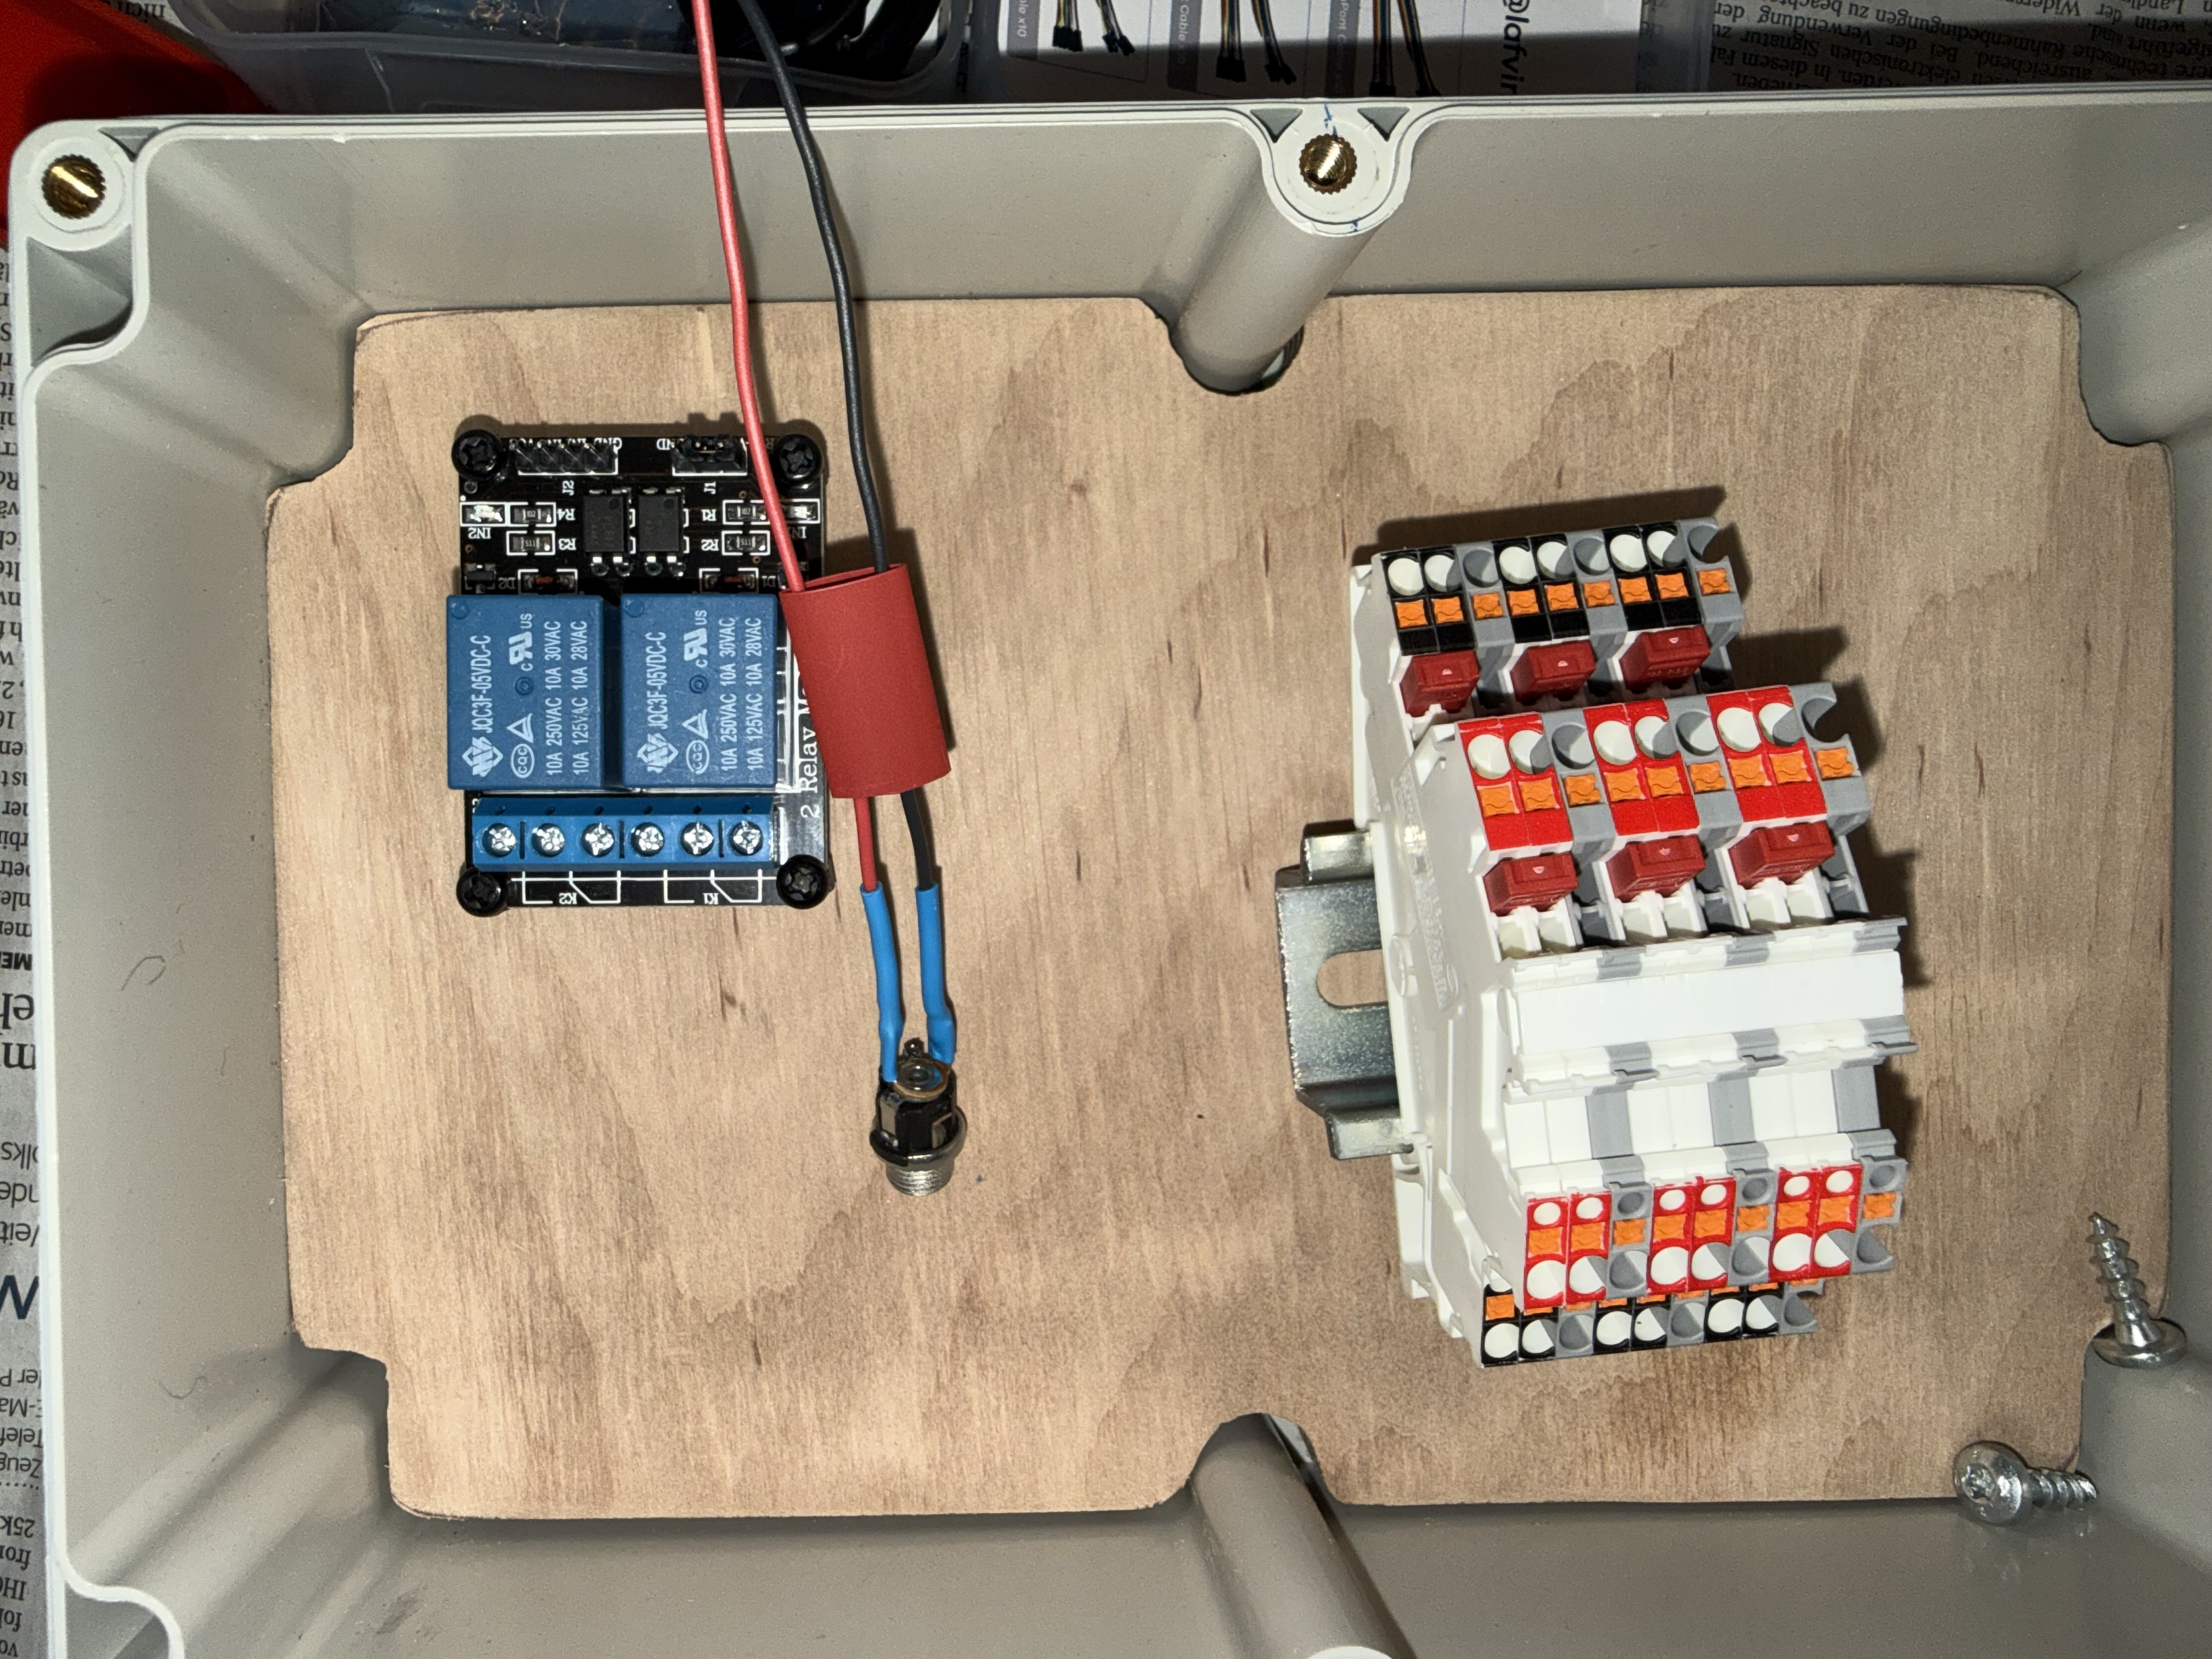
\includegraphics[width=\textwidth, height=5cm, keepaspectratio]{graphics/dev-7.jpeg}
        \caption{Soldering of connections}
        \label{fig:assembly_3}
    \end{subfigure}
    \hfill
    \begin{subfigure}[b]{0.45\textwidth}
        \centering
        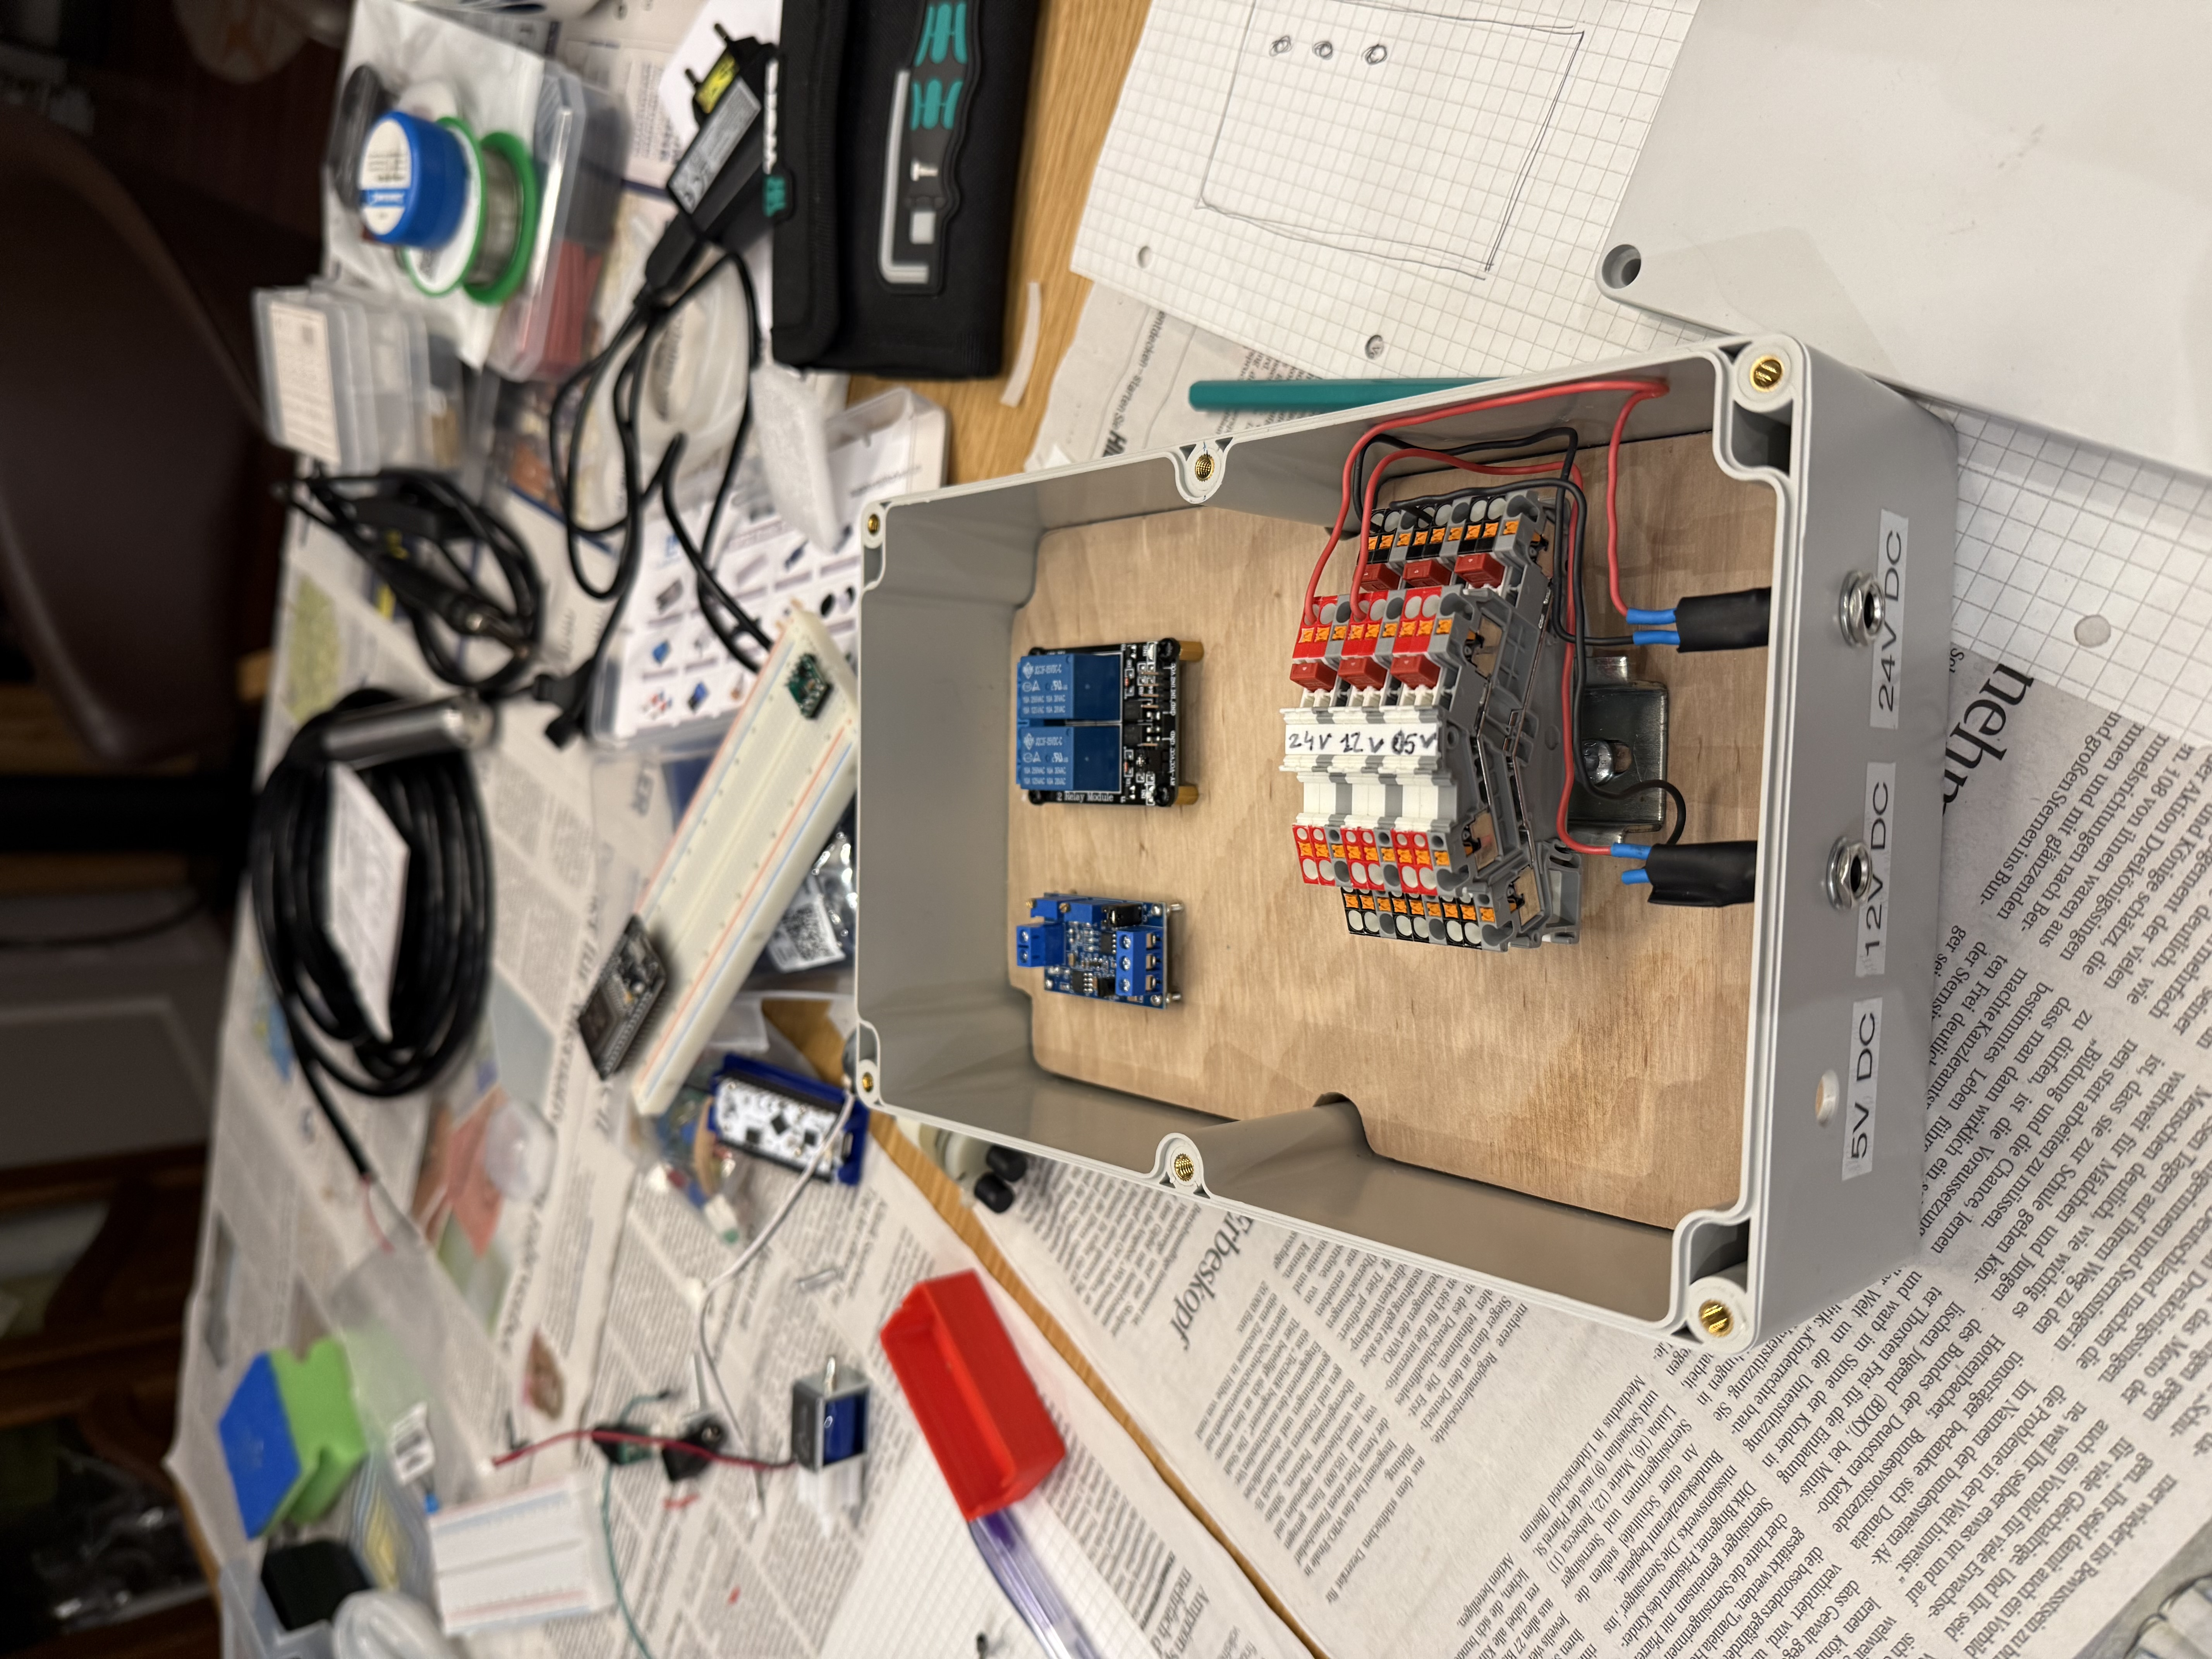
\includegraphics[width=\textwidth, height=5cm, angle=270]{graphics/dev-5.jpeg}
        \caption{Wiring terminal blocks}
        \label{fig:assembly_4}
    \end{subfigure}

    \vspace{1cm} 

    % --- ROW 3 ---
    \begin{subfigure}[b]{0.45\textwidth}
        \centering
        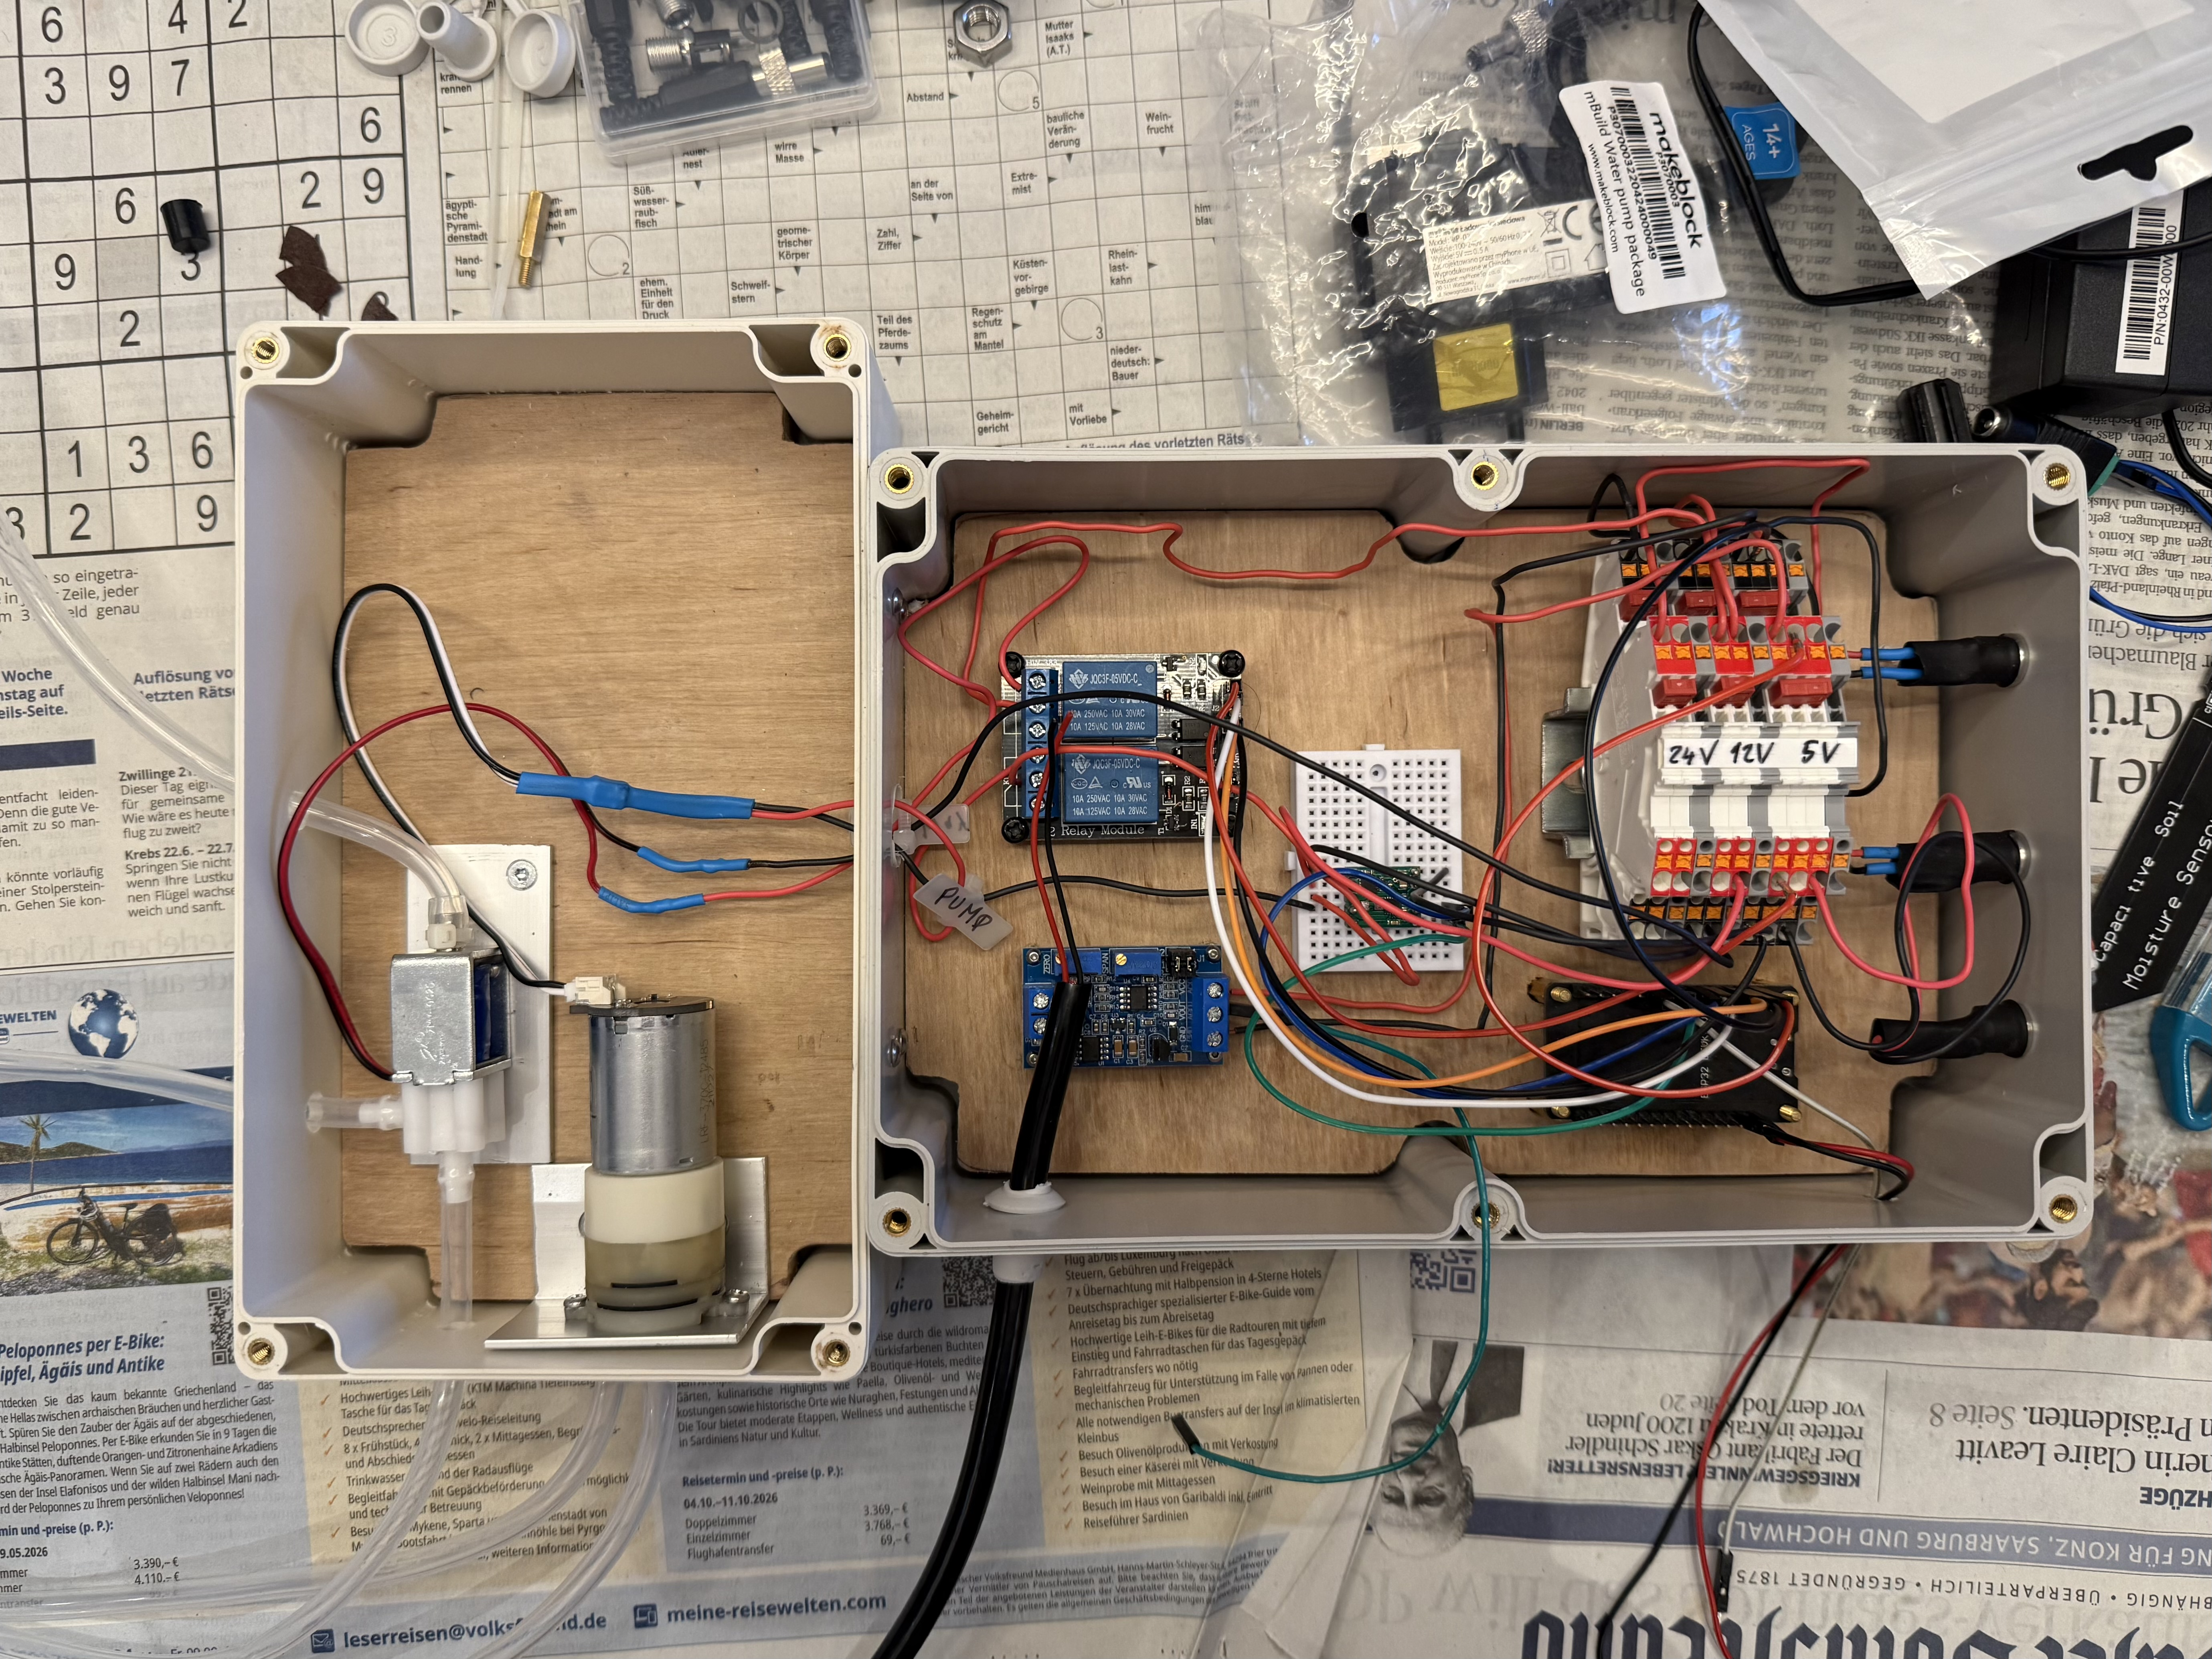
\includegraphics[width=\textwidth, height=5cm, keepaspectratio]{graphics/dev-6.jpeg}
        \caption{electrical wiring}
        \label{fig:assembly_5}
    \end{subfigure}
    \hfill
    \begin{subfigure}[b]{0.45\textwidth}
        \centering
        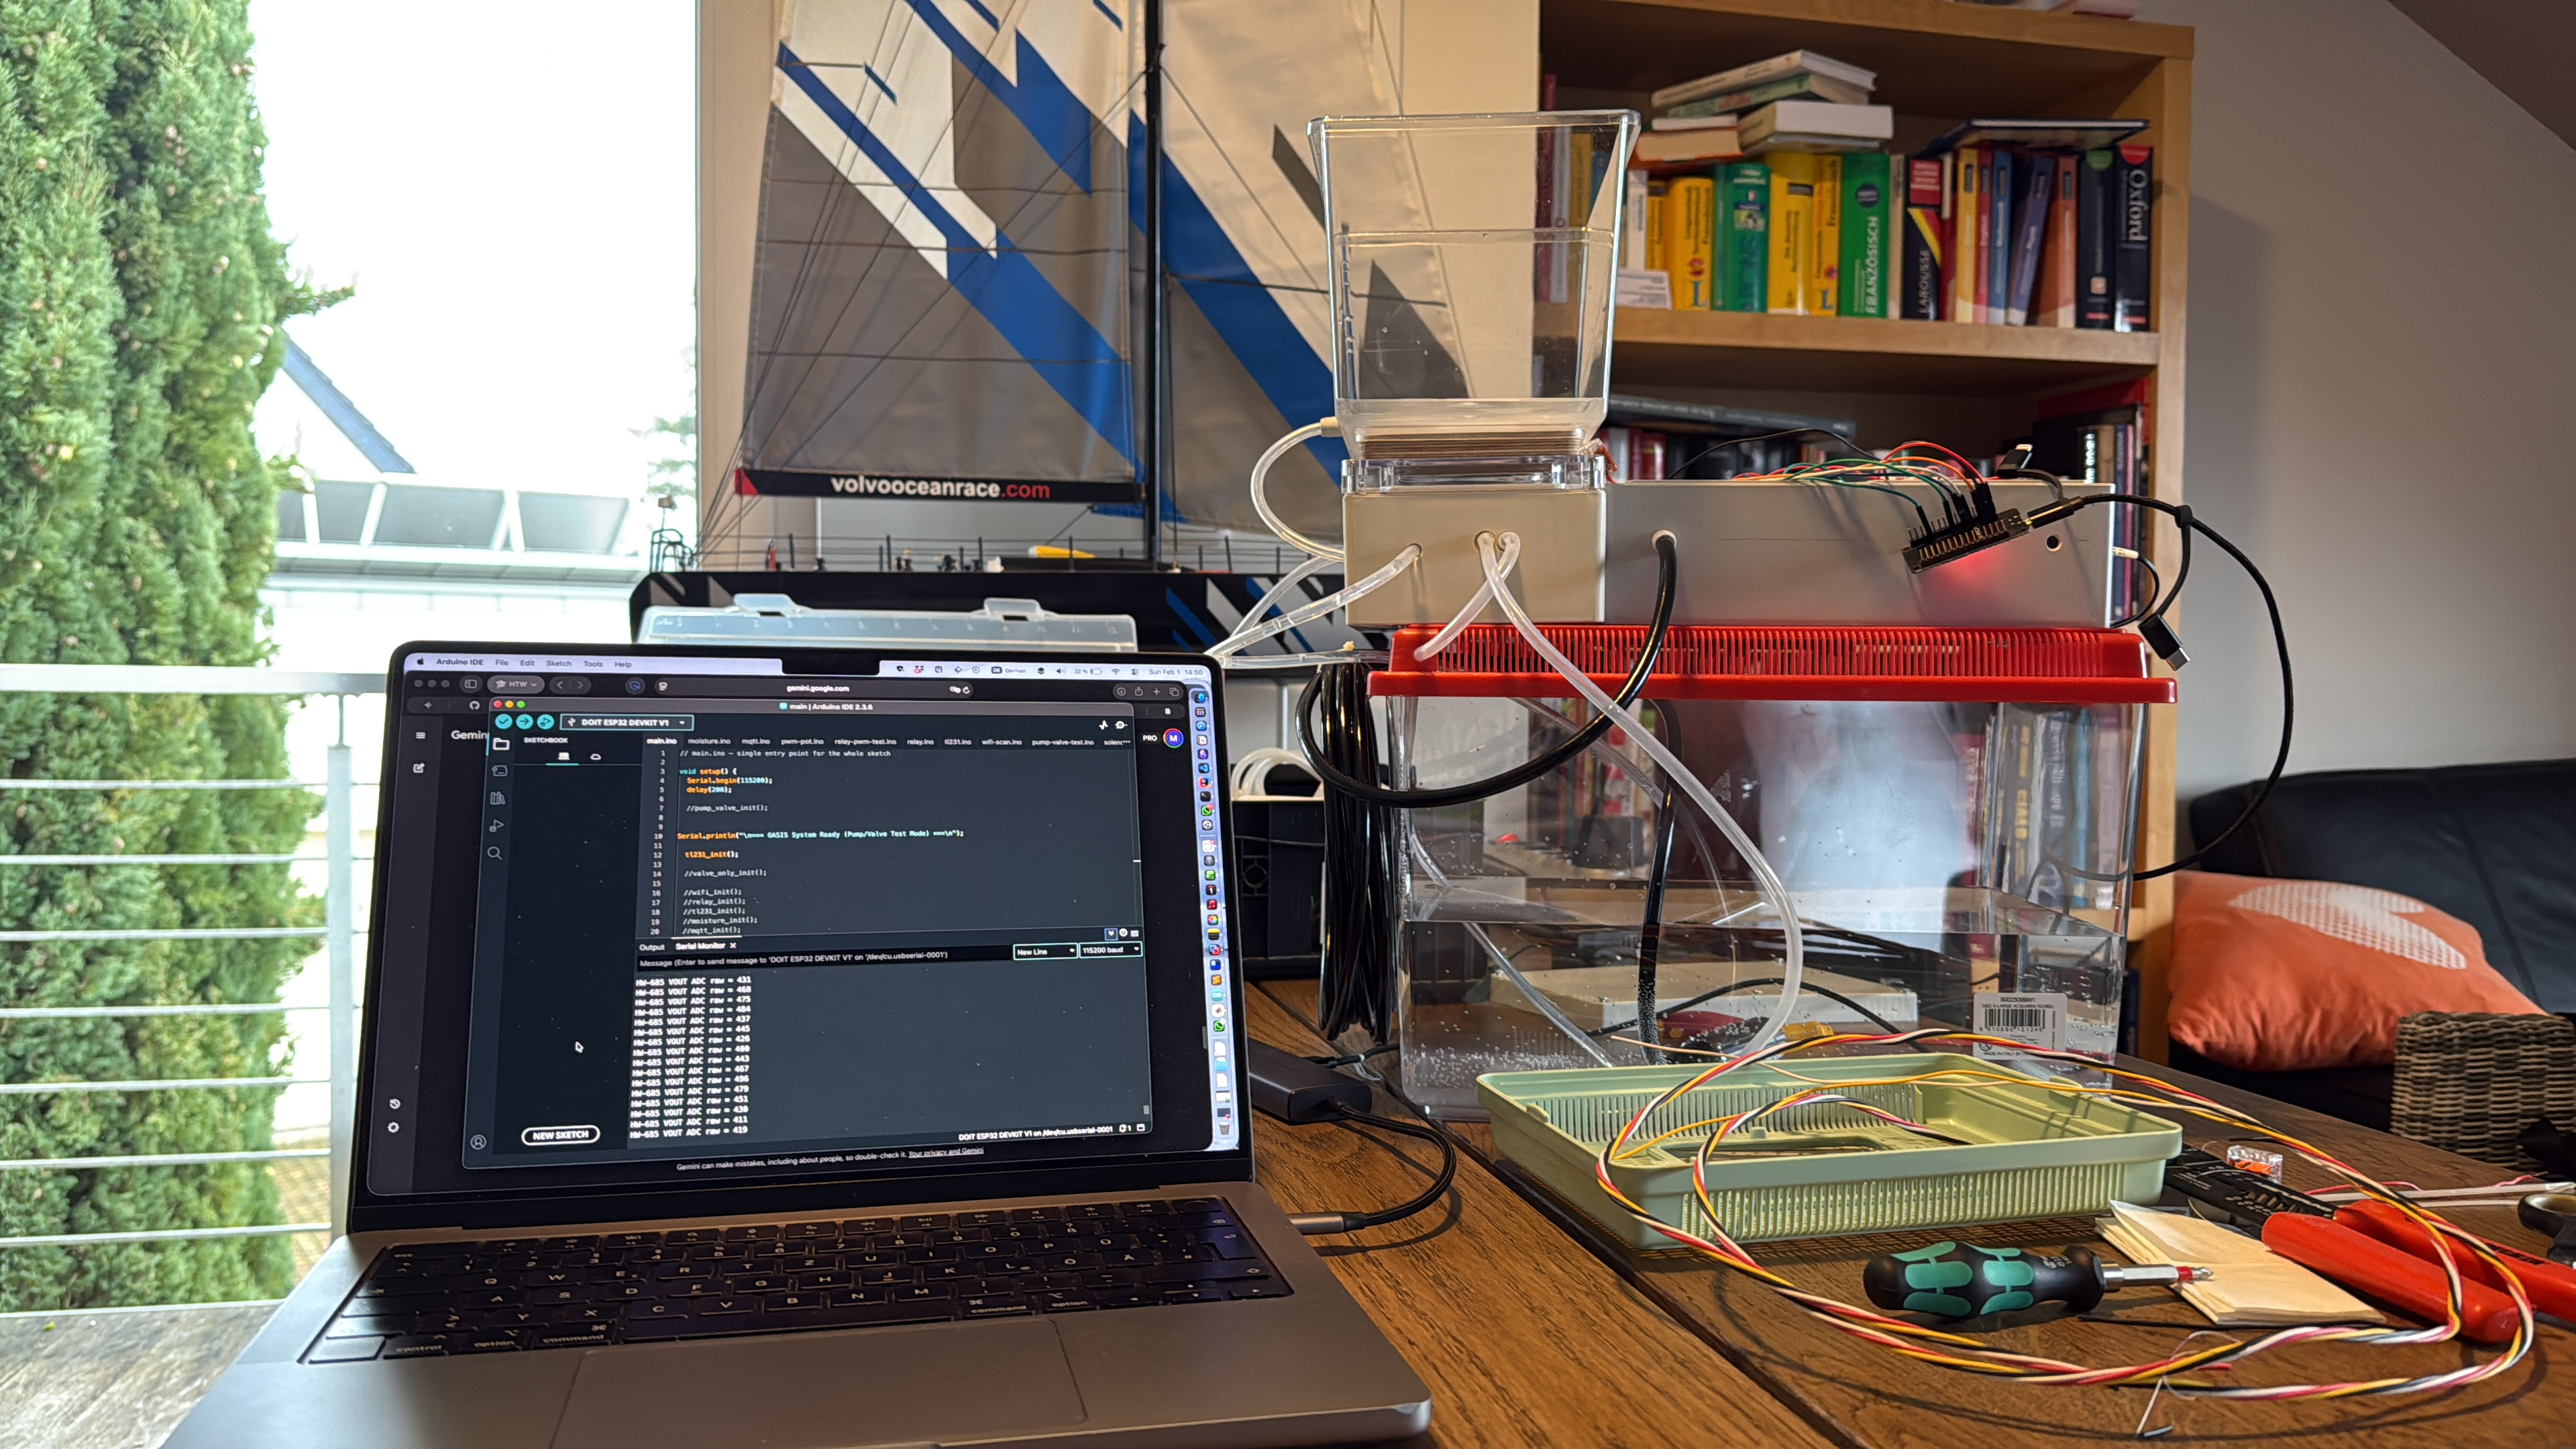
\includegraphics[width=\textwidth, height=5cm, keepaspectratio]{graphics/dev-12.jpg}
        \caption{finished project}
        \label{fig:assembly_6}
    \end{subfigure}
    
    \caption{Hardware Assembly Process (Part 2)}
    \label{fig:gallery_page1}
\end{figure}

\clearpage % Forces a page break for the next set of images

% --- REPEAT THE BLOCK ABOVE FOR PAGE 2 ---


\newpage
\subsection{Quotes / Citations}




\begin{itemize}
    
    \item \textbf{Turais Tech Docs}, \textit{Turais TL231 technical documentation}. Available at: \url{https://docs.turais.de/docs/sensors/misc/tl231-water-level-sensor/} \\
    (Accessed: \today).

    \item \textbf{Turais Tech Docs}, \textit{Turais HW-685 technical documentation}. Available at: \url{https://docs.turais.de/de/docs/modules/hw685/} \\(Accessed: \today).
    
    \item \textbf{Polulu Docs}, \textit{Polulu MAX14870 technical documentation}. Available at: \url{https://www.pololu.com/product/2961} \\
    (Accessed: \today).

    \item \textbf{Circuit State Docs}, \textit{Curcuit State ESP32 technical documentation}. Available at: \url{https://www.circuitstate.com/pinouts/doit-esp32-devkit-v1-wifi-development-board-pinout-diagram-and-reference/} \\
    (Accessed: \today).

    
    \item \textbf{How to Mechatronics: }\textit{YouTube tutorial on Controlling a DC Motor using an H-Bridge}. Available at: \url{https://www.youtube.com/watch?v=I7IFsQ4tQU8} \\
    (Accessed: \today).
    
\end{itemize}

\subsection{AI Tools}

During the development of this project, Generative AI Tools like ChatGPT and Gemini were used as supportive resources. They were primarily used for debugging, optimizing syntax and clarifying technical concepts.

\clearpage
\appendix
\end{document}

